\examtitle{CSD203_SU26_FE}
\examconfig{duration=60; audio_play_limit=1}
\section{s1}{Lý thuyết và Thuật toán Cấu trúc Dữ liệu}

\begin{question}{1}{mcq}
\source{Q1.webp}
\prompt{In a Red-Black tree, what is the color of the root?}
\choice{A}{Red}
\choice{B}{Black}
\choice{C}{Either Red or Black}
\choice{D}{Leaf color depends}
\answer{B}
\confidence{high}
\evidence{Property 2 of Red-Black Trees explicitly states: The root node is always black.}
\explain{- **Hướng giải**:
  Nhắc lại 5 tính chất cơ bản cấu thành Cây Đỏ-Đen (Red-Black Tree).

- **Các bước giải chi tiết / Phân tích**:
  1. Cây Đỏ-Đen là cây tìm kiếm nhị phân tự cân bằng với các quy tắc tô màu nút:
     - Tính chất 1: Mỗi nút chỉ có màu đỏ hoặc đen.
     - Tính chất 2 (Root Property): Nút gốc luôn luôn là màu đen (The root is black).
     - Tính chất 3: Tất cả các lá ảo (NIL / null leaves) đều là màu đen.
     - Tính chất 4 (Red Property): Nếu một nút có màu đỏ, thì cả hai con của nó đều phải là màu đen (không có hai nút đỏ kề nhau).
     - Tính chất 5 (Black-Height Property): Mọi đường đi đơn từ một nút đến các lá con cháu đều chứa số lượng nút đen bằng nhau.
  2. Do đó, nút gốc bắt buộc phải có màu đen.

- **Kiểm tra lại**:
  Khớp hoàn toàn với phương án B.

- **Vì sao các phương án khác sai**:
  - **A. Red**: Vi phạm trực tiếp tính chất 2 của cây Đỏ-Đen.
  - **C. Either Red or Black**: Sai, gốc không bao giờ được phép là màu đỏ.
  - **D. Leaf color depends**: Sai, lá luôn là đen.

- **Ghi nhớ / Công thức**:
  - Quy tắc bất biến của Red-Black Tree: Gốc luôn đen (Root is Black), Lá luôn đen (Leaves are Black).}
\end{question}

\begin{question}{2}{mcq}
\source{Q2.webp}
\prompt{What is the minimum number of nodes in a binary tree of height h?}
\choice{A}{h - 1}
\choice{B}{h + 1}
\choice{C}{h}
\choice{D}{2^h - 1}
\answer{B}
\confidence{high}
\evidence{When height h is defined as the number of edges on the longest path from root to leaf (root at height 0), a binary tree must have at least 1 node at each level from 0 to h, yielding at least h + 1 nodes (e.g., a degenerate/skewed chain of nodes).}
\explain{- **Hướng giải**:
  Xác định số lượng nút tối thiểu (minimum number of nodes) trong cây nhị phân có chiều cao \(h\).

- **Các bước giải chi tiết / Phân tích**:
  1. Theo quy ước chuẩn trong giáo trình cấu trúc dữ liệu (Adam Drozdek), chiều cao \(h\) của cây là số cạnh của đường đi dài nhất từ gốc tới một nút lá.
     - Cây có 1 nút duy nhất (nút gốc): chiều cao \(h = 0\), số nút \(n = 1 = h + 1\).
     - Cây có 2 nút nối nhau bởi 1 cạnh: chiều cao \(h = 1\), số nút \(n = 2 = h + 1\).
  2. Để số nút đạt tối thiểu với chiều cao \(h\), tại mỗi tầng (mức từ \(0\) đến \(h\)) chỉ cần đúng 1 nút duy nhất (cây lệch hoàn toàn - skewed/degenerate binary tree).
  3. Số tầng từ \(0\) đến \(h\) là \(h + 1\) tầng, do đó số nút tối thiểu là \(n_{\min} = h + 1\).

- **Kiểm tra lại**:
  - Số nút tối đa: \(n_{\max} = 2^{h+1} - 1\).
  - Số nút tối thiểu: \(n_{\min} = h + 1\).
  - Khớp với đáp án B.

- **Vì sao các phương án khác sai**:
  - **A. h - 1**: Quá nhỏ, không thể tạo được đường đi độ dài \(h\).
  - **C. h**: Chỉ đúng nếu quy ước gốc ở mức 1 (nhưng khi đó cây 1 nút có \(h = 1\) nút, cây 0 nút có \(h = 0\); câu hỏi này theo chuẩn FPTU với số cạnh \(h\) cho ra \(h + 1\)).
  - **D. 2^h - 1**: Đây là số nút tối đa của cây nhị phân khi gốc ở mức 1 hoặc số nút của cây đầy đủ chiều cao \(h - 1\).

- **Ghi nhớ / Công thức**:
  - Cây nhị phân chiều cao \(h\) (cạnh): \(n_{\min} = h + 1\); \(n_{\max} = 2^{h+1} - 1\).}
\end{question}

\begin{question}{3}{mcq}
\source{Q3.webp}
\prompt{For implementing a task scheduler where tasks are processed by priority, which of the following is ideal?}
\choice{A}{Tree}
\choice{B}{Heap}
\choice{C}{Stack}
\choice{D}{Queue}
\answer{B}
\confidence{high}
\evidence{A Heap (specifically a Priority Queue implemented with a Binary Heap) provides optimal O(log n) insertion and O(log n) extraction of the highest-priority task, making it the ideal choice for priority-based task scheduling.}
\explain{- **Hướng giải**:
  Xác định cấu trúc dữ liệu tối ưu nhất để quản lý các tác vụ xử lý theo mức độ ưu tiên (Priority Task Scheduler).

- **Các bước giải chi tiết / Phân tích**:
  1. Trong hệ thống điều phối tác vụ theo ưu tiên (Task Scheduler by Priority), mỗi tác vụ đi kèm một mức độ ưu tiên (priority value).
  2. Hệ thống cần hai thao tác thường xuyên:
     - Thêm một tác vụ mới vào bộ lập lịch.
     - Lấy tác vụ có mức độ ưu tiên cao nhất ra để CPU thực thi trước.
  3. Cấu trúc Đống nhị phân (Binary Heap / Priority Queue) hỗ trợ:
     - Lấy phần tử ưu tiên cao nhất (gốc đống): \(O(1)\).
     - Xóa phần tử ưu tiên cao nhất: \(O(\log n)\).
     - Thêm tác vụ mới: \(O(\log n)\).
  4. Do đó, Heap là cấu trúc dữ liệu lý tưởng và chuẩn mực nhất cho bộ lập lịch theo độ ưu tiên.

- **Kiểm tra lại**:
  Khớp hoàn toàn với phương án B.

- **Vì sao các phương án khác sai**:
  - **A. Tree**: Cây tổng quát không đảm bảo việc lấy max/min nhanh chóng nếu không cân bằng.
  - **C. Stack**: Hoạt động LIFO, phục vụ lưu lịch sử/quay lui, không theo độ ưu tiên.
  - **D. Queue**: Hàng đợi thông thường hoạt động FIFO (đến trước phục vụ trước), không hỗ trợ độ ưu tiên.

- **Ghi nhớ / Công thức**:
  - Priority Scheduling \(\rightarrow\) Priority Queue \(\rightarrow\) Binary Heap (Min-Heap / Max-Heap).}
\end{question}

\begin{question}{4}{mcq}
\source{Q4.webp}
\prompt{Given the following pseudo code for a binary tree structure, what is the output of the inorder traversal?
\begin{code}{python}
root = TreeNode('R')
root.left = nodeA
root.right = nodeB

nodeA.left = nodeC
nodeA.right = nodeD

nodeB.left = nodeE
nodeB.right = nodeF

nodeF.left = nodeG
\end{code}}
\choice{A}{C A D R E B G F}
\choice{B}{C D A B E G F R}
\choice{C}{C A D R E G F B}
\choice{D}{G F E B R D A C}
\answer{A}
\confidence{high}
\evidence{Inorder traversal is Left -> Root -> Right. Left subtree of R is A with children C, D -> Inorder is C A D. Root is R. Right subtree of R is B: Left child is E; B is root; Right child is F whose left child is G -> Inorder is E B G F. Concatenating: C A D R E B G F.}
\explain{- **Hướng giải**:
  Dựng cấu trúc cây nhị phân từ mã gán liên kết và thực hiện phép duyệt Trung thứ tự (In-order: Left - Node - Right).

- **Các bước giải chi tiết / Phân tích**:
  1. Phân tích cấu trúc cây:
     - Nút gốc là `R`.
     - Cây con trái của `R` là `A`:
       - `A.left = C`, `A.right = D`.
       - Cây con của `C` và `D` rỗng (lá).
     - Cây con phải của `R` là `B`:
       - `B.left = E`.
       - `B.right = F`.
       - `F.left = G` (F không có con phải, G là lá).
  2. Duyệt In-order (Trái \(\rightarrow\) Gốc \(\rightarrow\) Phải):
     - Duyệt cây con trái của `R` (gốc `A`):
       - Inorder(`A`) = `C` \(\rightarrow\) `A` \(\rightarrow\) `D`.
     - Thăm nút gốc: `R`.
     - Duyệt cây con phải của `R` (gốc `B`):
       - Con trái của `B` là `E`.
       - Thăm nút `B`.
       - Con phải của `B` là `F`: duyệt con trái của `F` là `G` \(\rightarrow\) thăm `F`.
       - Kết quả nhánh phải: `E` \(\rightarrow\) `B` \(\rightarrow\) `G` \(\rightarrow\) `F`.
  3. Ghép toàn bộ chuỗi: `C A D R E B G F`.

- **Kiểm tra lại**:
  Khớp chính xác từng ký tự với phương án A.

- **Vì sao các phương án khác sai**:
  - **B**: Thứ tự sai nhánh phải và đặt R ở cuối (dạng post-order).
  - **C**: `E G F B` sai vị trí nút B (B phải đứng trước cây con phải của nó).
  - **D**: Thứ tự duyệt ngược hoàn toàn.

- **Ghi nhớ / Công thức**:
  - In-order: Duyệt đệ quy cây con trái \(\rightarrow\) Thăm nút gốc \(\rightarrow\) Duyệt đệ quy cây con phải.}
\end{question}

\begin{question}{5}{mcq}
\source{Q5.webp}
\prompt{Which of the following is a disadvantage of AVL trees?}
\choice{A}{They are not balanced}
\choice{B}{They require additional space for storing balance factors}
\choice{C}{They do not support in-order traversal}
\choice{D}{They are balanced}
\answer{B}
\confidence{high}
\evidence{Each node in an AVL tree must maintain its height or balance factor in order to perform rotations during insertion and deletion, requiring extra memory space per node.}
\explain{- **Hướng giải**:
  Xác định nhược điểm (disadvantage) của Cây AVL so với cây tìm kiếm nhị phân thông thường và các cây cân bằng khác.

- **Các bước giải chi tiết / Phân tích**:
  1. Cây AVL là cây nhị phân tự cân bằng nghiêm ngặt (chênh lệch chiều cao hai con không quá 1).
  2. Để duy trì tính chất này sau mỗi lần chèn hoặc xóa nút:
     - Mỗi nút trong cây AVL phải lưu trữ thêm chiều cao (height) hoặc hệ số cân bằng (balance factor = -1, 0, hoặc 1).
     - Trường dữ liệu phụ này tiêu tốn thêm bộ nhớ RAM cho từng nút trên cây (require additional space for storing balance factors).
     - Ngoài ra, việc cân bằng nghiêm ngặt đòi hỏi nhiều phép quay (rotations) hơn khi chèn/xóa.
  3. Như vậy, phương án B chỉ ra chính xác nhược điểm về không gian bộ nhớ của cây AVL.

- **Kiểm tra lại**:
  Khớp hoàn toàn với phương án B.

- **Vì sao các phương án khác sai**:
  - **A. They are not balanced**: Hoàn toàn sai, cây AVL luôn luôn cân bằng.
  - **C. They do not support in-order traversal**: Sai, cây AVL là một BST nên hỗ trợ duyệt in-order tăng dần bình thường.
  - **D. They are balanced**: Đây là ưu điểm vượt trội của cây AVL, không phải là nhược điểm.

- **Ghi nhớ / Công thức**:
  - Nhược điểm của AVL: Tốn bộ nhớ lưu trữ hệ số cân bằng và chi phí quay cây khi chèn/xóa nhiều.}
\end{question}

\begin{question}{6}{mcq}
\source{Q6.webp}
\prompt{(Choose 1 answer)
Given the sequential representation of the binary tree T in the figure where an one-dimensional array is used to store the elements of tree (the size of T is 16 and the root node of the tree T is the node at the index 1):

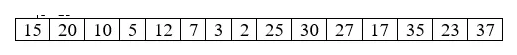
\includegraphics{assets/Q6_fig.png}

The ancestors of the node 30 are:}
\choice{A}{15, 20, 12}
\choice{B}{15, 20, 5}
\choice{C}{15, 10, 12}
\choice{D}{15, 20, 10}
\figdesc{Mảng 1 chiều biểu diễn cây nhị phân kích thước 16 với gốc 15 tại chỉ số 1: [15, 20, 10, 5, 12, 7, 3, 2, 25, 30, 27, 17, 35, 23, 37].}
\answer{A}
\confidence{high}
\evidence{In the array, root 15 is at index 1. Indices: 1:15, 2:20, 3:10, 4:5, 5:12, 6:7, 7:3, 8:2, 9:25, 10:30. Node 30 is at index 10. Parent of index 10 is 10 // 2 = 5 (node 12). Parent of index 5 is 5 // 2 = 2 (node 20). Parent of index 2 is 2 // 2 = 1 (node 15). The ancestors are 15, 20, 12.}
\explain{- **Hướng giải**:
  Áp dụng công thức quan hệ cha-con trong biểu diễn mảng 1 chiều 1-indexed của cây nhị phân để tìm các nút tổ tiên (ancestors) của nút có giá trị 30.

- **Các bước giải chi tiết / Phân tích**:
  1. Dãy mảng trong hình biểu diễn cây với gốc tại chỉ số 1:
     - Chỉ số 1: `15` (Gốc)
     - Chỉ số 2: `20`
     - Chỉ số 3: `10`
     - Chỉ số 4: `5`
     - Chỉ số 5: `12`
     - Chỉ số 6: `7`
     - Chỉ số 7: `3`
     - Chỉ số 8: `2`
     - Chỉ số 9: `25`
     - Chỉ số 10: `30`
  2. Nút có giá trị 30 nằm tại chỉ số \(i = 10\).
  3. Trong mảng 1-indexed, nút cha của nút tại chỉ số \(i\) nằm tại \(\lfloor i / 2 \rfloor\):
     - Cha của chỉ số 10: \(10 // 2 = 5\) \(\rightarrow\) giá trị nút là `12`.
     - Cha của chỉ số 5: \(5 // 2 = 2\) \(\rightarrow\) giá trị nút là `20`.
     - Cha của chỉ số 2: \(2 // 2 = 1\) \(\rightarrow\) giá trị nút là `15` (nút gốc).
  4. Tập hợp các nút tổ tiên (ancestors) từ gốc tới cha trực tiếp là: `15, 20, 12`.

- **Kiểm tra lại**:
  Khớp chính xác với phương án A.

- **Vì sao các phương án khác sai**:
  - **B**: Chứa số 5 (chỉ số 4, là anh em của nút 12, không phải cha của 10).
  - **C**: Chứa số 10 (chỉ số 3, thuộc nhánh con bên phải của gốc 15).
  - **D**: Chứa số 10.

- **Ghi nhớ / Công thức**:
  - Trong mảng 1-indexed: `parent(i) = i // 2`; `left(i) = 2*i`; `right(i) = 2*i + 1`.}
\end{question}

\begin{question}{7}{mcq}
\source{Q7.webp}
\prompt{If a binary tree has N nodes, how many edges does it have?}
\choice{A}{N - 1}
\choice{B}{N}
\choice{C}{N + 1}
\choice{D}{2N}
\answer{A}
\confidence{high}
\evidence{In any tree with N vertices (including binary trees), there are always exactly N - 1 edges because every node except the root has exactly one incoming edge from its parent.}
\explain{- **Hướng giải**:
  Áp dụng định lý cơ bản về số cạnh của một cây (Tree) trong Lý thuyết Đồ thị.

- **Các bước giải chi tiết / Phân tích**:
  1. Cây là một đồ thị liên thông không có chu trình (chu kỳ).
  2. Trong bất kỳ cây có gốc (rooted tree) nào có \(N\) đỉnh:
     - Nút gốc không có cạnh đi vào từ phía trên (không có nút cha).
     - Mọi nút còn lại trong \(N - 1\) nút đều có đúng 1 cạnh nối duy nhất đi từ nút cha của nó.
  3. Do đó, tổng số cạnh trong cây luôn luôn là \(N - 1\).
  4. Tính chất này đúng với mọi cây nhị phân có \(N\) nút.

- **Kiểm tra lại**:
  Ví dụ cây có 3 nút: số cạnh là \(3 - 1 = 2\). Khớp hoàn toàn với phương án A.

- **Vì sao các phương án khác sai**:
  - **B. N**: Một đồ thị liên thông có \(N\) đỉnh và \(N\) cạnh sẽ tạo thành đúng 1 chu trình (không còn là cây).
  - **C. N + 1**: Nhiều cạnh hơn cây, chắc chắn chứa chu trình.
  - **D. 2N**: Sai.

- **Ghi nhớ / Công thức**:
  - Với mọi cây có \(N\) nút: Số cạnh \(|E| = N - 1\).}
\end{question}

\begin{question}{8}{mcq}
\source{Q8.webp}
\prompt{You are given pointers to first node of a singly linked list, which of the following operations takes O(n) where n is the length of the linked list?}
\choice{A}{Delete the first element}
\choice{B}{Insert a new element as a first element}
\choice{C}{Add a new element at the end of the list}
\choice{D}{None of these}
\answer{C}
\confidence{high}
\evidence{Without a tail pointer, inserting at the end of a singly linked list requires traversing all n nodes from the head to reach the last node, which takes O(n) time.}
\explain{- **Hướng giải**:
  Phân tích độ phức tạp thời gian của các thao tác trên Danh sách liên kết đơn khi chỉ có con trỏ trỏ tới nút đầu tiên (`head`).

- **Các bước giải chi tiết / Phân tích**:
  1. Xét thao tác thêm phần tử vào cuối danh sách (Add a new element at the end of the list):
     - Vì đề bài chỉ cho con trỏ trỏ tới phần tử đầu tiên (pointer to first node) và không có con trỏ `tail`.
     - Để thêm vào cuối, ta buộc phải duyệt tuần tự từ `head` qua từng nút cho đến khi gặp nút cuối cùng (nút có `next == None`).
     - Thao tác duyệt này phải đi qua \(n\) phần tử, mất thời gian tỉ lệ thuận với độ dài danh sách \(\rightarrow O(n)\).
  2. Xét các thao tác còn lại:
     - Xóa phần tử đầu tiên: Cập nhật `head = head.next` mất \(O(1)\).
     - Chèn phần tử mới vào đầu: `new_node.next = head; head = new_node` mất \(O(1)\).
  3. Vậy thao tác mất \(O(n)\) là thêm phần tử vào cuối danh sách.

- **Kiểm tra lại**:
  Khớp hoàn toàn với phương án C.

- **Vì sao các phương án khác sai**:
  - **A, B**: Đều thực hiện tại vị trí `head`, chỉ cần cập nhật con trỏ trong thời gian hằng số \(O(1)\).
  - **D**: Sai vì phương án C là đáp án đúng.

- **Ghi nhớ / Công thức**:
  - Singly Linked List (chỉ có head): Thao tác ở đầu = \(O(1)\); Thao tác ở cuối = \(O(n)\).}
\end{question}

\begin{question}{9}{mcq}
\source{Q9.webp}
\prompt{What is a Singly Linked List?}
\choice{A}{A data structure where elements are stored in a linear sequence and each element points to the next one.}
\choice{B}{A data structure where elements are stored in a random sequence and each element points to the next one.}
\choice{C}{A data structure where elements are stored in a tree-like structure.}
\choice{D}{A data structure where elements are stored in a stack-like structure.}
\answer{A}
\confidence{high}
\evidence{A singly linked list is a linear data structure where elements are arranged in a linear sequence and each node points to the subsequent node.}
\explain{- **Hướng giải**:
  Nhắc lại định nghĩa chuẩn về Danh sách liên kết đơn (Singly Linked List).

- **Các bước giải chi tiết / Phân tích**:
  1. Danh sách liên kết đơn là một cấu trúc dữ liệu tuyến tính (linear data structure).
  2. Trong cấu trúc này, các phần tử (nodes) tạo thành một chuỗi thứ tự tuyến tính logic (linear sequence).
  3. Mỗi phần tử chứa giá trị dữ liệu và một con trỏ trỏ tới phần tử kế tiếp duy nhất trong chuỗi (each element points to the next one).

- **Kiểm tra lại**:
  Khớp hoàn toàn với phương án A.

- **Vì sao các phương án khác sai**:
  - **B**: "random sequence" (chuỗi ngẫu nhiên) là sai, các nút có thứ tự xác định rõ ràng.
  - **C**: Cấu trúc cây (tree-like) là cấu trúc phi tuyến tính phân nhánh, không phải danh sách liên kết đơn.
  - **D**: Stack-like chỉ là cách thức truy xuất LIFO, không phải định nghĩa tổng quát của SLL.

- **Ghi nhớ / Công thức**:
  - Singly Linked List = Linear collection where each node links to its successor.}
\end{question}

\begin{question}{10}{mcq}
\source{Q10.webp}
\prompt{Which array operation takes O(1) time complexity?}
\choice{A}{Inserting at the front}
\choice{B}{Removing an element}
\choice{C}{Indexing an element}
\choice{D}{Growing the array}
\answer{C}
\confidence{high}
\evidence{Indexing an element in an array takes O(1) constant time due to direct pointer arithmetic: base_address + index * element_size.}
\explain{- **Hướng giải**:
  Xác định thao tác có độ phức tạp thời gian hằng số \(O(1)\) trên cấu trúc dữ liệu mảng (Array).

- **Các bước giải chi tiết / Phân tích**:
  1. Mảng cấp phát các ô nhớ liên tiếp nhau.
  2. Thao tác truy xuất theo chỉ số (Indexing an element): Trình biên dịch tính toán trực tiếp địa chỉ ô nhớ bằng phép nhân và cộng số học trong \(O(1)\).
  3. Các thao tác khác trên mảng:
     - Chèn ở đầu (Inserting at front): phải dời các phần tử sang phải \(\rightarrow O(n)\).
     - Xóa phần tử (Removing an element): phải dời các phần tử sang trái \(\rightarrow O(n)\).
     - Mở rộng mảng (Growing array): phải cấp phát vùng nhớ mới và sao chép mảng \(\rightarrow O(n)\).
  4. Do đó, chỉ có Indexing an element là có độ phức tạp \(O(1)\).

- **Kiểm tra lại**:
  Khớp hoàn toàn với phương án C.

- **Vì sao các phương án khác sai**:
  - **A, B, D**: Đều mất chi phí dịch chuyển hoặc sao chép \(O(n)\).

- **Ghi nhớ / Công thức**:
  - Mảng cho phép truy cập ngẫu nhiên (Random Access) trong \(O(1)\).}
\end{question}

\begin{question}{11}{mcq}
\source{Q11.webp}
\prompt{What additional memory does a doubly linked list require per node compared to a singly linked list?}
\choice{A}{1 pointer}
\choice{B}{2 pointers}
\choice{C}{3 pointers}
\choice{D}{0 pointer}
\answer{A}
\confidence{high}
\evidence{A singly linked list node has 1 pointer (next). A doubly linked list node has 2 pointers (next and prev). The difference is exactly 1 additional pointer per node.}
\explain{- **Hướng giải**:
  So sánh kích thước bộ nhớ của một nút trong Danh sách liên kết đôi (DLL) so với Danh sách liên kết đơn (SLL).

- **Các bước giải chi tiết / Phân tích**:
  1. Cấu trúc một nút trong Singly Linked List gồm:
     - 1 trường dữ liệu (`data`).
     - 1 con trỏ trỏ tới nút kế tiếp (`next`).
  2. Cấu trúc một nút trong Doubly Linked List gồm:
     - 1 trường dữ liệu (`data`).
     - 1 con trỏ trỏ tới nút kế tiếp (`next`).
     - 1 con trỏ trỏ tới nút phía trước (`prev`).
  3. So sánh phần bộ nhớ bổ sung (additional memory per node): DLL chỉ cần thêm duy nhất 1 con trỏ (`prev`).

- **Kiểm tra lại**:
  Khớp hoàn toàn với phương án A.

- **Vì sao các phương án khác sai**:
  - **B. 2 pointers**: DLL có tổng cộng 2 con trỏ, nhưng phần bộ nhớ cần thêm (additional) so với SLL chỉ là 1 con trỏ.
  - **C. 3 pointers**: Sai.
  - **D. 0 pointer**: Sai, DLL chắc chắn tốn nhiều bộ nhớ hơn SLL.

- **Ghi nhớ / Công thức**:
  - Dung lượng thêm của DLL trên mỗi nút = 1 pointer (kích thước thường là 4 bytes trên kiến trúc 32-bit hoặc 8 bytes trên kiến trúc 64-bit).}
\end{question}

\begin{question}{12}{mcq}
\source{Q12.webp}
\prompt{In a circularly linked list with n nodes, how can you efficiently check if the list is circular when given only a pointer to the head node?}
\choice{A}{Traverse the entire list and check if any node's next pointer points back to the head.}
\choice{B}{Use two pointers, where one moves faster than the other, and check if they meet}
\choice{C}{Count the number of nodes in the list and compare it to a predefined value.}
\choice{D}{Check the tail node directly to see if its next pointer points to the head}
\answer{B}
\confidence{high}
\evidence{Floyd's Cycle-Finding Algorithm (tortoise and hare) uses two pointers moving at different speeds to detect cycles or circularity in O(n) time and O(1) auxiliary space without modifying the list.}
\explain{- **Hướng giải**:
  Nhận diện giải thuật tối ưu và kinh điển để phát hiện danh sách có cấu trúc vòng hay không (Cycle Detection).

- **Các bước giải chi tiết / Phân tích**:
  1. Khi chỉ được cung cấp một con trỏ tới nút đầu (`head`), danh sách có thể là danh sách liên kết đơn có đuôi `None`, hoặc có chu trình vòng ở giữa, hoặc là danh sách vòng tròn hoàn chỉnh.
  2. Thuật toán phát hiện chu trình Floyd (Floyd's Cycle-Finding Algorithm / Tortoise and Hare):
     - Sử dụng hai con trỏ: con trỏ rùa (chậm, đi 1 bước) và con trỏ thỏ (nhanh, đi 2 bước).
     - Nếu danh sách có vòng, con trỏ nhanh chắc chắn sẽ đuổi kịp và gặp lại con trỏ chậm (they meet).
     - Nếu danh sách không có vòng, con trỏ nhanh sẽ chạm tới `None`.
  3. Kỹ thuật này hoạt động trong thời gian \(O(n)\) và không tốn thêm bộ nhớ ngoài (\(O(1)\) không gian).

- **Kiểm tra lại**:
  Khớp hoàn toàn với phương án B.

- **Vì sao các phương án khác sai**:
  - **A**: Nếu danh sách có một chu trình không quay về head (ví dụ hình chữ P / lasso), duyệt kiểm tra về head sẽ bị lặp vô tận.
  - **C**: Không thể đếm số nút nếu chưa biết danh sách có dừng hay không.
  - **D**: Đề bài chỉ cho con trỏ `head`, không có sẵn con trỏ trực tiếp tới nút `tail`.

- **Ghi nhớ / Công thức**:
  - Thuật toán hai con trỏ (Floyd's algorithm): con trỏ chậm và con trỏ nhanh gặp nhau \(\rightarrow\) danh sách có chu trình.}
\end{question}

\begin{question}{13}{mcq}
\source{Q13.webp}
\prompt{In Linked List implementation, a node carries information regarding_______}
\choice{A}{Data}
\choice{B}{Link}
\choice{C}{Data and Link}
\choice{D}{Node}
\answer{C}
\confidence{high}
\evidence{Each node in a linked list contains at least two essential fields: the actual payload (Data) and a reference to another node (Link).}
\explain{- **Hướng giải**:
  Xác định các thông tin thiết yếu mà một nút trong danh sách liên kết lưu trữ.

- **Các bước giải chi tiết / Phân tích**:
  1. Cấu trúc của một nút (node) trong mọi danh sách liên kết gồm:
     - Trường thông tin dữ liệu (`Data` / `info`): lưu giá trị phần tử.
     - Trường liên kết (`Link` / `next` / `pointer`): lưu địa chỉ tham chiếu tới nút tiếp theo.
  2. Do đó, một nút mang đầy đủ thông tin về cả Dữ liệu và Liên kết (Data and Link).

- **Kiểm tra lại**:
  Khớp hoàn toàn với phương án C.

- **Vì sao các phương án khác sai**:
  - **A. Data**: Chỉ đúng một nửa, thiếu trường liên kết.
  - **B. Link**: Chỉ đúng một nửa, thiếu dữ liệu.
  - **D. Node**: Nút không chỉ chứa "nút", mà chứa dữ liệu và liên kết.

- **Ghi nhớ / Công thức**:
  - Cấu tạo Node = Data field + Link (Pointer) field.}
\end{question}

\begin{question}{14}{mcq}
\source{Q14.webp}
\prompt{How to remove an element x after element y of a non-empty singly linked list?}
\choice{A}{y.next = x.next}
\choice{B}{x.next = y.next;}
\choice{C}{head.next = x}
\choice{D}{head.next = y}
\answer{A}
\confidence{high}
\evidence{To bypass and delete node x (which currently equals y.next), the next pointer of y must be updated to point directly to node x's next successor: y.next = x.next.}
\explain{- **Hướng giải**:
  Xác định phép gán con trỏ để xóa nút \(x\) đứng ngay sau nút \(y\) trong danh sách liên kết đơn.

- **Các bước giải chi tiết / Phân tích**:
  1. Ban đầu, chuỗi liên kết có thứ tự: \(y \rightarrow x \rightarrow x.\text{next}\).
  2. Để loại bỏ nút \(x\) ra khỏi chuỗi liên kết, ta cần nối tắt liên kết từ \(y\) bỏ qua \(x\) và trỏ thẳng tới nút đứng sau \(x\).
  3. Nút đứng sau \(x\) là `x.next`.
  4. Do đó, lệnh cập nhật là: `y.next = x.next`.
  5. Sau lệnh này, \(x\) bị tách khỏi danh sách và có thể được giải phóng bộ nhớ (garbage collected).

- **Kiểm tra lại**:
  Khớp hoàn toàn với phương án A.

- **Vì sao các phương án khác sai**:
  - **B. x.next = y.next**: Gán sai chiều, không làm thay đổi liên kết trong danh sách.
  - **C, D**: Sửa con trỏ của `head`, làm đứt gãy phần đầu danh sách.

- **Ghi nhớ / Công thức**:
  - Xóa nút sau `y`: `y.next = y.next.next` (hoặc `y.next = x.next` với `x = y.next`).}
\end{question}

\begin{question}{15}{mcq}
\source{Q15.webp}
\prompt{In a circularly linked list, what does the next pointer of the last node point to?}
\choice{A}{NULL}
\choice{B}{The head node}
\choice{C}{The previous node}
\choice{D}{Itself}
\answer{B}
\confidence{high}
\evidence{By definition, the last node of a circular linked list points back to the first node (the head node), forming a closed loop.}
\explain{- **Hướng giải**:
  Nhắc lại định nghĩa cốt lõi của Danh sách liên kết vòng (Circular Linked List).

- **Các bước giải chi tiết / Phân tích**:
  1. Khác với danh sách liên kết tuyến tính thông thường nơi nút cuối cùng trỏ tới `NULL` / `None`.
  2. Trong danh sách liên kết vòng, nút cuối cùng (last node / tail) có con trỏ `next` trỏ ngược trở lại nút đầu tiên của danh sách (The head node).
  3. Nhờ đó, việc duyệt danh sách tạo thành một chu trình khép kín.

- **Kiểm tra lại**:
  Khớp hoàn toàn với phương án B.

- **Vì sao các phương án khác sai**:
  - **A. NULL**: Đây là đặc điểm của danh sách liên kết đơn thông thường.
  - **C. The previous node**: Sai, liên kết ngược là con trỏ `prev` trong danh sách đôi.
  - **D. Itself**: Chỉ xảy ra khi danh sách vòng chỉ có duy nhất 1 nút.

- **Ghi nhớ / Công thức**:
  - Danh sách vòng: `tail.next == head`.}
\end{question}

\begin{question}{16}{mcq}
\source{Q16.webp}
\prompt{What is the load factor in a hash table?}
\choice{A}{The number of keys divided by the number of buckets}
\choice{B}{The number of buckets divided by the number of keys}
\choice{C}{The size of the hash value}
\choice{D}{The total number of entries}
\answer{A}
\confidence{high}
\evidence{The load factor alpha of a hash table is defined as alpha = n / m, where n is the number of keys (entries) and m is the number of buckets (table capacity).}
\explain{- **Hướng giải**:
  Nhắc lại công thức định nghĩa hệ số tải (Load Factor) trong cấu trúc dữ liệu Bảng băm.

- **Các bước giải chi tiết / Phân tích**:
  1. Hệ số tải (thường ký hiệu là \(\alpha\)) thể hiện mức độ lấp đầy trung bình của các ô trong bảng băm.
  2. Công thức toán học:
     \[ \alpha = \frac{n}{m} \]
     - Trong đó: \(n\) là số lượng phần tử / khóa đã chèn vào bảng (number of keys/entries).
     - \(m\) là tổng số ô chứa / dung lượng của bảng băm (number of buckets/slots).
  3. Do đó, hệ số tải là số lượng khóa chia cho số lượng ô chứa (The number of keys divided by the number of buckets).

- **Kiểm tra lại**:
  Khớp hoàn toàn với phương án A.

- **Vì sao các phương án khác sai**:
  - **B**: Đảo ngược tỉ số (buckets chia cho keys).
  - **C**: Kích thước giá trị băm là số nguyên, không phải tỉ số.
  - **D**: Tổng số phần tử chỉ là tử số \(n\), không phải hệ số tải.

- **Ghi nhớ / Công thức**:
  - Load factor: \(\alpha = \frac{\text{Số phần tử (n)}}{\text{Số ô chứa (m)}}\).}
\end{question}

\begin{question}{17}{mcq}
\source{Q17.webp}
\prompt{In the context of hash tables, what is the load factor?}
\choice{A}{The ratio of the number of entries in the hash table to the table's capacity.}
\choice{B}{The number of collisions that occur during hash table operations.}
\choice{C}{A measure of the efficiency of the hash function.}
\choice{D}{The number of elements that can be stored in a single bucket.}
\answer{A}
\confidence{high}
\evidence{Load factor is the ratio of stored elements (entries) to the total table size (capacity).}
\explain{- **Hướng giải**:
  Hiểu bản chất định nghĩa hệ số tải (Load Factor) dưới dạng tỉ số dung lượng.

- **Các bước giải chi tiết / Phân tích**:
  1. Trong bảng băm, hệ số tải \(\alpha = n / m\) là tỉ số giữa số mục dữ liệu hiện có trong bảng (number of entries) so với tổng dung lượng sức chứa của bảng (table's capacity).
  2. Khi hệ số tải vượt quá một ngưỡng nhất định (ví dụ 0.75 trong Java HashMap), bảng băm sẽ thực hiện tái băm (rehashing) để mở rộng kích thước nhằm duy trì tốc độ truy xuất \(O(1)\).
  3. Phát biểu A định nghĩa chính xác bản chất tỉ số này.

- **Kiểm tra lại**:
  Khớp hoàn toàn với phương án A.

- **Vì sao các phương án khác sai**:
  - **B**: Số lượng va chạm là một hệ quả khi hệ số tải tăng cao, không phải là định nghĩa hệ số tải.
  - **C**: Hệ số tải đo độ đầy của bảng, không đo trực tiếp chất lượng hàm băm.
  - **D**: Số phần tử trong 1 bucket liên quan đến độ dài danh sách liên kết trong separate chaining.

- **Ghi nhớ / Công thức**:
  - Load factor = Ratio of entries to capacity.}
\end{question}

\begin{question}{18}{mcq}
\source{Q18.webp}
\prompt{Select the correct statement about "hash collision".}
\choice{A}{It occurs when the hash function produces the same hash code for two different keys.}
\choice{B}{It is the process of resizing the hash table to accommodate more elements.}
\choice{C}{It is a mechanism to prevent unauthorized access to hash tables.}
\choice{D}{It is the process of inserting elements into the hash table.}
\answer{A}
\confidence{high}
\evidence{A hash collision happens whenever a hash function maps two distinct keys to the same index/code: h(k1) == h(k2) with k1 != k2.}
\explain{- **Hướng giải**:
  Nhắc lại định nghĩa chính xác của hiện tượng va chạm băm ("hash collision").

- **Các bước giải chi tiết / Phân tích**:
  1. Va chạm băm (Hash collision) xảy ra khi có hai khóa khác nhau (\(k_1 \neq k_2\)) mà hàm băm lại tạo ra cùng một mã băm / chỉ số ô lưu trữ giống nhau (\(h(k_1) = h(k_2)\)).
  2. Đây là một hiện tượng tự nhiên không thể tránh khỏi trong bảng băm do tập khóa có thể có kích thước lớn hơn nhiều so với kích thước bảng băm (theo Nguyên lý lồng chim bồ câu - Pigeonhole Principle).
  3. Do đó, phương án A mô tả hoàn hảo hiện tượng này.

- **Kiểm tra lại**:
  Khớp hoàn toàn với phương án A.

- **Vì sao các phương án khác sai**:
  - **B**: Quá trình thay đổi kích thước bảng gọi là Rehashing.
  - **C**: Không liên quan đến cơ chế bảo mật.
  - **D**: Thao tác chèn phần tử gọi là Insertion.

- **Ghi nhớ / Công thức**:
  - Collision: \(k_1 \neq k_2\) nhưng \(h(k_1) = h(k_2)\).}
\end{question}

\begin{question}{19}{mcq}
\source{Q19.webp}
\prompt{A hash function h defined h(key)=key mod 6, linear probing is used to insert the keys 1, 6, 11 into a hash table with size = 6. What will the location of key 12 be?}
\choice{A}{0}
\choice{B}{1}
\choice{C}{2}
\choice{D}{3}
\answer{C}
\confidence{high}
\evidence{Table size = 6. Insert 1: 1%6=1 (slot 1). Insert 6: 6%6=0 (slot 0). Insert 11: 11%6=5 (slot 5). Insert 12: 12%6=0 (collision at 0). Probe (0+1)%6=1 (collision at 1). Probe (0+2)%6=2 (empty -> placed at 2).}
\explain{- **Hướng giải**:
  Mô phỏng chi tiết từng bước chèn các khóa vào bảng băm kích thước \(m = 6\) với hàm băm \(h(\text{key}) = \text{key} \pmod 6\) và xử lý va chạm bằng dò tuyến tính (linear probing).

- **Các bước giải chi tiết / Phân tích**:
  1. Bảng băm có kích thước 6 (các chỉ số từ 0 đến 5 ban đầu đều rỗng).
  2. Chèn khóa 1:
     - \[ h(1) = 1 \pmod 6 = 1 \]
     - Ô 1 trống \(\rightarrow\) đặt khóa 1 vào ô 1.
  3. Chèn khóa 6:
     - \[ h(6) = 6 \pmod 6 = 0 \]
     - Ô 0 trống \(\rightarrow\) đặt khóa 6 vào ô 0.
  4. Chèn khóa 11:
     - \[ h(11) = 11 \pmod 6 = 5 \]
     - Ô 5 trống \(\rightarrow\) đặt khóa 11 vào ô 5.
  5. Bây giờ chèn khóa 12:
     - \[ h(12) = 12 \pmod 6 = 0 \]
     - Ô 0 đã bị khóa 6 chiếm giữ (xảy ra va chạm).
     - Dò tuyến tính ô kế tiếp \(i = 1\): \((0 + 1) \pmod 6 = 1\) \(\rightarrow\) ô 1 đã bị khóa 1 chiếm giữ.
     - Dò tuyến tính ô kế tiếp \(i = 2\): \((0 + 2) \pmod 6 = 2\) \(\rightarrow\) ô 2 hiện đang trống!
     - Đặt khóa 12 vào ô 2.
  6. Vậy vị trí của khóa 12 là chỉ số 2.

- **Kiểm tra lại**:
  - Trạng thái bảng băm sau khi chèn 12: `[0: 6, 1: 1, 2: 12, 3: empty, 4: empty, 5: 11]`.
  - Khóa 12 ở vị trí 2. Khớp với phương án C.

- **Vì sao các phương án khác sai**:
  - **A. 0**: Ô 0 đã có phần tử 6.
  - **B. 1**: Ô 1 đã có phần tử 1.
  - **D. 3**: Chỉ số 3 trống nhưng đứng sau chỉ số 2 nên thuật toán dừng ngay tại ô 2.

- **Ghi nhớ / Công thức**:
  - Dò tuyến tính: \(h(k, i) = (h(k) + i) \pmod m\).}
\end{question}

\begin{question}{20}{mcq}
\source{Q20.webp}
\prompt{Which of the following method is not a collision resolution strategy for open addressing in hash tables?}
\choice{A}{Linear probing.}
\choice{B}{Quadratic probing.}
\choice{C}{Double hashing.}
\choice{D}{Chaining.}
\answer{D}
\confidence{high}
\evidence{Chaining (separate chaining) stores colliding elements outside the primary table slots via auxiliary linked lists, classifying it as closed addressing. Open addressing includes Linear probing, Quadratic probing, and Double hashing.}
\explain{- **Hướng giải**:
  Phân loại các chiến lược giải quyết xung đột băm giữa Băm mở (Open Addressing) và Băm đóng (Chaining / Closed Addressing).

- **Các bước giải chi tiết / Phân tích**:
  1. Trong Bảng băm, có hai họ phương pháp xử lý va chạm chính:
     - **Băm mở (Open Addressing)**: Mọi phần tử đều được lưu trữ trực tiếp ngay bên trong mảng bảng băm. Khi va chạm, tìm một ô trống khác theo một chuỗi dò cố định:
       - Dò tuyến tính (Linear Probing)
       - Dò bậc hai (Quadratic Probing)
       - Băm kép (Double Hashing)
     - **Băm nối kết (Separate Chaining / Closed Addressing)**: Mỗi ô trong bảng băm trỏ tới một cấu trúc dữ liệu ngoài (thường là danh sách liên kết) để lưu trữ các phần tử trùng vị trí.
  2. Do đó, Chaining không thuộc về Open Addressing.

- **Kiểm tra lại**:
  Khớp hoàn toàn với phương án D.

- **Vì sao các phương án khác sai**:
  - **A, B, C**: Đều là 3 phương pháp tiêu biểu cấu thành Open Addressing.

- **Ghi nhớ / Công thức**:
  - Open Addressing: Mọi khóa nằm trong bảng (Linear probing, Quadratic probing, Double hashing).
  - Closed Addressing / Chaining: Khóa nằm trong danh sách liên kết ngoài.}
\end{question}

\begin{question}{21}{mcq}
\source{Q21.webp}
\prompt{What is the time complexity for inserting a new node at the beginning of a singly linked list?}
\choice{A}{O(1)}
\choice{B}{O(n)}
\choice{C}{O(log n)}
\choice{D}{O(n log n)}
\answer{A}
\confidence{high}
\evidence{Prepending to a singly linked list only requires setting new_node.next = head and head = new_node, which involves a constant number of pointer assignments taking O(1) time.}
\explain{- **Hướng giải**:
  Phân tích số lượng thao tác cần thiết để chèn một nút mới vào vị trí đầu tiên của danh sách liên kết đơn.

- **Các bước giải chi tiết / Phân tích**:
  1. Để chèn một nút mới `new_node` vào đầu danh sách liên kết đơn có con trỏ `head`:
     - Gán con trỏ của nút mới trỏ tới `head` hiện tại: `new_node.next = head`.
     - Cập nhật lại con trỏ `head`: `head = new_node`.
  2. Cả hai thao tác này chỉ là phép gán con trỏ đơn giản, không phụ thuộc vào độ dài \(n\) của danh sách.
  3. Thời gian thực thi là hằng số \(O(1)\).

- **Kiểm tra lại**:
  Khớp hoàn toàn với phương án A.

- **Vì sao các phương án khác sai**:
  - **B. O(n)**: Là chi phí khi chèn vào cuối danh sách nếu không có con trỏ `tail`.
  - **C. O(log n)**: Độ phức tạp của chèn trên cây cân bằng, không phải danh sách liên kết.
  - **D. O(n log n)**: Độ phức tạp của sắp xếp.

- **Ghi nhớ / Công thức**:
  - Thao tác chèn/xóa ở đầu danh sách liên kết luôn là \(O(1)\).}
\end{question}

\begin{question}{22}{mcq}
\source{Q22.webp}
\prompt{What is the function of the following pseudocode?

\begin{code}{text}
Algorithm Traversal(G, u):
Input: A graph G and a vertex u of G
Output: A collection of vertices reachable from u, with their discovery edges

for each outgoing edge e = (u, v) of u do
    if vertex v has not been visited then
        Mark vertex v as visited (via edge e).
        Recursively call Traversal(G, v).
\end{code}}
\choice{A}{It performs a breadth-first search (BFS) starting from vertex u.}
\choice{B}{It performs a depth-first search (DFS) starting from vertex u.}
\choice{C}{It finds the shortest path from u to all other vertices.}
\choice{D}{It detects cycles in the graph starting from vertex u.}
\answer{B}
\confidence{high}
\evidence{The pseudocode explores edges outgoing from u and immediately recursively calls Traversal(G, v) on unvisited neighbors, which is the canonical recursive implementation of Depth-First Search (DFS).}
\explain{- **Hướng giải**:
  Đọc hiểu mã giả thuật toán duyệt đồ thị và nhận diện cơ chế đệ quy chiều sâu.

- **Các bước giải chi tiết / Phân tích**:
  1. Thuật toán nhận vào đồ thị \(G\) và đỉnh bắt đầu \(u\).
  2. Với mỗi cạnh đi ra \(e = (u, v)\), nếu đỉnh \(v\) chưa thăm, thuật toán đánh dấu đã thăm và gọi đệ quy `Traversal(G, v)` ngay lập tức.
  3. Cơ chế gọi đệ quy đi sâu vào từng nhánh trước khi quay lại các đỉnh lân cận khác chính là bản chất của Thuật toán Tìm kiếm theo chiều sâu (Depth-First Search - DFS).

- **Kiểm tra lại**:
  Khớp hoàn toàn với phương án B.

- **Vì sao các phương án khác sai**:
  - **A. BFS**: Tìm kiếm theo chiều rộng dùng Hàng đợi (Queue) lặp theo từng lớp mức, không dùng đệ quy trực tiếp.
  - **C. Shortest path**: DFS không đảm bảo tìm đường đi ngắn nhất trên đồ thị có trọng số.
  - **D. Cycle detection**: Mặc dù DFS có thể được ứng dụng để phát hiện chu trình, mục tiêu chính của đoạn mã là duyệt các đỉnh tới được từ \(u\).

- **Ghi nhớ / Công thức**:
  - DFS đặc trưng bởi cấu trúc Ngăn xếp / Đệ quy (LIFO).
  - BFS đặc trưng bởi cấu trúc Hàng đợi (FIFO).}
\end{question}

\begin{question}{23}{mcq}
\source{Q23.webp}
\prompt{The data structure required for Breadth First Traversal on a graph is?}
\choice{A}{Stack}
\choice{B}{Queue}
\choice{C}{Array}
\choice{D}{Linked list}
\answer{B}
\confidence{high}
\evidence{Breadth-First Search (BFS) processes vertices level-by-level in First-In, First-Out order, fundamentally requiring a Queue data structure.}
\explain{- **Hướng giải**:
  Xác định cấu trúc dữ liệu cốt lõi phục vụ thuật toán duyệt đồ thị theo chiều rộng (BFS).

- **Các bước giải chi tiết / Phân tích**:
  1. Thuật toán duyệt theo chiều rộng (Breadth-First Traversal - BFS) duyệt các đỉnh theo từng lớp khoảng cách từ đỉnh gốc (level by level).
  2. Để đảm bảo các đỉnh ở mức gần được thăm và xử lý trước các đỉnh ở mức xa hơn, các đỉnh kề được đưa vào một cấu trúc hàng chờ theo nguyên tắc Vào trước - Ra trước (FIFO - First In First Out).
  3. Cấu trúc dữ liệu cài đặt cơ chế FIFO này chính là Hàng đợi (Queue).

- **Kiểm tra lại**:
  Khớp hoàn toàn với phương án B.

- **Vì sao các phương án khác sai**:
  - **A. Stack**: Dùng cho duyệt theo chiều sâu (DFS).
  - **C. Array**: Mảng chỉ là bộ lưu trữ tổng quát, không cung cấp cơ chế FIFO nếu không cài hàng đợi.
  - **D. Linked list**: Có thể dùng để cài đặt queue, nhưng cấu trúc dữ liệu trừu tượng cần thiết là Queue.

- **Ghi nhớ / Công thức**:
  - BFS \(\rightarrow\) Queue (FIFO).
  - DFS \(\rightarrow\) Stack / Recursion (LIFO).}
\end{question}

\begin{question}{24}{mcq}
\source{Q24.webp}
\prompt{What is the suitable data structure used in Dijkstra's algorithm to manage distances during traversal?}
\choice{A}{Priority queue}
\choice{B}{Hash table}
\choice{C}{Stack}
\choice{D}{Binary tree}
\answer{A}
\confidence{high}
\evidence{Dijkstra's algorithm greedily extracts the unvisited vertex with minimum tentative distance at each step, making a Min-Priority Queue (Binary Heap / Fibonacci Heap) the optimal data structure.}
\explain{- **Hướng giải**:
  Xác định cấu trúc dữ liệu thích hợp nhất để quản lý và trích xuất khoảng cách tạm thời nhỏ nhất trong thuật toán Dijkstra.

- **Các bước giải chi tiết / Phân tích**:
  1. Thuật toán Dijkstra tìm đường đi ngắn nhất từ một đỉnh nguồn tới tất cả các đỉnh khác trên đồ thị có trọng số không âm.
  2. Tại mỗi bước lặp, thuật toán cần chọn ra đỉnh chưa thăm có khoảng cách ước lượng \(d[u]\) là nhỏ nhất (minimum distance).
  3. Sau đó, thuật toán cập nhật khoảng cách tới các đỉnh kề (relax edges).
  4. Để thực hiện thao tác lấy đỉnh có khoảng cách nhỏ nhất (`extract-min`) và cập nhật khoảng cách (`decrease-key`) một cách hiệu quả nhất trong \(O(\log V)\), cấu trúc Hàng đợi ưu tiên (Priority Queue - Min-Heap) là lựa chọn chuẩn mực và tối ưu nhất.
  5. Nhờ đó độ phức tạp của thuật toán giảm xuống \(O((V + E) \log V)\).

- **Kiểm tra lại**:
  Khớp hoàn toàn với phương án A.

- **Vì sao các phương án khác sai**:
  - **B. Hash table**: Tra cứu theo khóa trong \(O(1)\) nhưng không hỗ trợ tìm min nhanh chóng (mất \(O(V)\)).
  - **C. Stack**: Hoạt động LIFO, không thể lấy phần tử có khoảng cách nhỏ nhất.
  - **D. Binary tree**: Cây tổng quát không chuyên dụng bằng Priority Queue.

- **Ghi nhớ / Công thức**:
  - Dijkstra + Min-Priority Queue (Min-Heap) \(\rightarrow\) Thời gian \(O((V + E) \log V)\).}
\end{question}

\begin{question}{25}{mcq}
\source{Q25.webp}
\prompt{Given a set V = {V1, V2, ... Vn} of n vertices, how many undirected graphs (not necessarily connected) can be constructed out of V?}
\choice{A}{n(n - 1)/2}
\choice{B}{2^n}
\choice{C}{n!}
\choice{D}{2^(n(n - 1)/2)}
\answer{D}
\confidence{high}
\evidence{In an undirected graph with n vertices, there are C(n, 2) = n(n - 1)/2 possible edges. Each edge can either be present or absent (2 choices), yielding 2^(n(n - 1)/2) possible graphs.}
\explain{- **Hướng giải**:
  Áp dụng công thức tổ hợp đếm số lượng đồ thị vô hướng có thể tạo thành từ tập \(n\) đỉnh phân biệt.

- **Các bước giải chi tiết / Phân tích**:
  1. Cho tập đỉnh gồm \(n\) đỉnh phân biệt \(V = \{V_1, V_2, \dots, V_n\}\).
  2. Một cạnh vô hướng là một cặp gồm 2 đỉnh phân biệt không kể thứ tự. Tổng số cạnh tối đa có thể có giữa \(n\) đỉnh là tổ hợp chập 2 của \(n\):
     \[ M = \binom{n}{2} = \frac{n(n - 1)}{2} \]
  3. Với mỗi cạnh tiềm năng trong số \(M\) cạnh này, ta có đúng 2 khả năng độc lập: cạnh đó có tồn tại trong đồ thị hoặc không tồn tại (có hoặc không).
  4. Theo quy tắc nhân của giải tích tổ hợp, tổng số đồ thị vô hướng khác nhau có thể tạo thành là:
     \[ 2^M = 2^{\frac{n(n - 1)}{2}} \]

- **Kiểm tra lại**:
  - Ví dụ với \(n = 3\): \(M = 3 \times 2 / 2 = 3\). Số đồ thị là \(2^3 = 8\).
  - Khớp với đáp án D: `2^(n(n-1)/2)`.

- **Vì sao các phương án khác sai**:
  - **A. n(n-1)/2**: Đây là số cạnh tối đa của đồ thị đầy đủ \(K_n\), không phải số lượng đồ thị.
  - **B. 2^n**: Số tập con của tập đỉnh.
  - **C. n!**: Số hoán vị của \(n\) đỉnh.

- **Ghi nhớ / Công thức**:
  - Số đồ thị vô hướng từ \(n\) đỉnh: \(2^{\binom{n}{2}} = 2^{n(n - 1)/2}\).
  - Số đồ thị có hướng từ \(n\) đỉnh: \(2^{n(n - 1)}\).}
\end{question}

\begin{question}{26}{mcq}
\source{Q26.webp}
\prompt{(Choose 1 answer)
What is the shortest path from node A to node G?

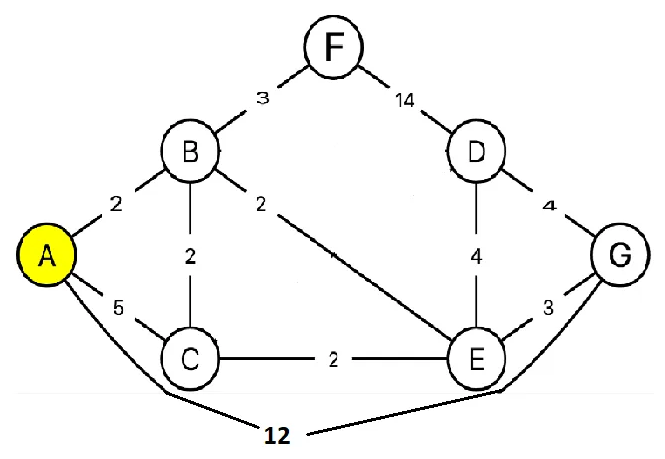
\includegraphics{assets/Q26_fig.png}}
\choice{A}{A-C-E-G}
\choice{B}{A-B-E-G}
\choice{C}{A-G}
\choice{D}{A-B-C-E-G}
\figdesc{Đồ thị có trọng số gồm các đỉnh A, B, C, D, E, F, G với trọng số các cạnh: A-B: 2, A-C: 5, A-G: 12, B-C: 2, B-F: 3, B-E: 2, C-E: 2, F-D: 14, E-D: 4, D-G: 4, E-G: 3.}
\answer{B}
\confidence{high}
\evidence{Evaluating candidate paths from A to G in figure: Path A-G has weight 12. Path A-C-E-G has weight 5 + 2 + 3 = 10. Path A-B-C-E-G has weight 2 + 2 + 2 + 3 = 9. Path A-B-E-G has weight 2 + 2 + 3 = 7. Minimum cost is 7 via A-B-E-G.}
\explain{- **Hướng giải**:
  Áp dụng thuật toán tìm đường đi ngắn nhất (Dijkstra) để tính chi phí của các đường đi từ đỉnh A tới đỉnh G trên đồ thị có trọng số.

- **Các bước giải chi tiết / Phân tích**:
  1. Đọc trọng số các cạnh trên hình vẽ:
     - \(A - B = 2\), \(A - C = 5\), \(A - G = 12\).
     - \(B - C = 2\), \(B - F = 3\), \(B - E = 2\).
     - \(C - E = 2\).
     - \(F - D = 14\), \(E - D = 4\).
     - \(D - G = 4\), \(E - G = 3\).
  2. Tính tổng trọng số của các phương án đường đi từ A đến G:
     - Đường đi **A-G**: \(\text{chi phí} = 12\).
     - Đường đi **A-C-E-G**: \(\text{chi phí} = 5 + 2 + 3 = 10\).
     - Đường đi **A-B-C-E-G**: \(\text{chi phí} = 2 + 2 + 2 + 3 = 9\).
     - Đường đi **A-B-E-G**: \(\text{chi phí} = 2 + 2 + 3 = 7\).
  3. So sánh các chi phí: \(7 < 9 < 10 < 12\).
  4. Vậy đường đi ngắn nhất từ A đến G là **A-B-E-G** với tổng độ dài bằng 7.

- **Kiểm tra lại**:
  Khớp chính xác với phương án B.

- **Vì sao các phương án khác sai**:
  - **A. A-C-E-G**: Chi phí là 10 (lớn hơn 7 do đi qua cạnh AC có trọng số 5).
  - **C. A-G**: Chi phí là 12 (lớn hơn 7).
  - **D. A-B-C-E-G**: Chi phí là 9 (dư cạnh BC).

- **Ghi nhớ / Công thức**:
  - Đường đi ngắn nhất không nhất thiết phải có ít cạnh nhất (A-G có 1 cạnh nhưng chi phí 12, trong khi A-B-E-G có 3 cạnh nhưng chi phí chỉ là 7).}
\end{question}

\begin{question}{27}{mcq}
\source{Q27.webp}
\prompt{A graph in which exists a path between any two nodes is called}
\choice{A}{Complete graph}
\choice{B}{Connected graph}
\choice{C}{Digraph}
\choice{D}{In-directed graph}
\answer{B}
\confidence{high}
\evidence{A graph is defined as connected if every pair of vertices is joined by at least one path.}
\explain{- **Hướng giải**:
  Nhắc lại định nghĩa đồ thị liên thông (Connected Graph).

- **Các bước giải chi tiết / Phân tích**:
  1. Trong lý thuyết đồ thị, đồ thị vô hướng được gọi là liên thông (Connected graph) nếu giữa hai nút bất kỳ trong đồ thị luôn luôn tồn tại một đường đi (path).
  2. Nếu có ít nhất một cặp đỉnh không thể đi tới nhau được, đồ thị bị mất tính liên thông và tạo thành nhiều thành phần liên thông riêng biệt.

- **Kiểm tra lại**:
  Khớp hoàn toàn với phương án B.

- **Vì sao các phương án khác sai**:
  - **A. Complete graph**: Yêu cầu giữa mọi cặp đỉnh đều có cạnh trực tiếp (edge), không chỉ là đường đi (path).
  - **C. Digraph**: Đồ thị có hướng.
  - **D. In-directed graph**: Không phải thuật ngữ chuẩn.

- **Ghi nhớ / Công thức**:
  - Tồn tại đường đi giữa mọi cặp đỉnh = Connected graph.}
\end{question}

\begin{question}{28}{mcq}
\source{Q28.webp}
\prompt{Which method is not a part of the Queue module in Python?}
\choice{A}{put()}
\choice{B}{get()}
\choice{C}{push()}
\choice{D}{empty()}
\answer{C}
\confidence{high}
\evidence{In Python's built-in queue.Queue module, the primary insertion method is put(), extraction is get(), status checks include empty(), full(), qsize(). There is no push() method.}
\explain{- **Hướng giải**:
  Xác định giao diện phương thức (API methods) của lớp `queue.Queue` trong thư viện chuẩn của Python.

- **Các bước giải chi tiết / Phân tích**:
  1. Module `queue` trong thư viện chuẩn Python cung cấp lớp `Queue` đồng bộ hóa đa luồng với các phương thức chính:
     - `put(item)`: Thêm một phần tử vào hàng đợi (tương đương enqueue).
     - `get()`: Lấy và xóa một phần tử khỏi hàng đợi (tương đương dequeue).
     - `empty()`: Kiểm tra hàng đợi có rỗng không (trả về `True`/`False`).
     - `full()`: Kiểm tra hàng đợi có đầy không.
     - `qsize()`: Trả về số lượng phần tử.
  2. Lớp `Queue` không có phương thức nào tên là `push()` (`push` là thuật ngữ quen thuộc trong C++ `std::queue` hoặc `std::stack`, nhưng Python dùng `put`).
  3. Vì vậy, `push()` không thuộc module Queue trong Python.

- **Kiểm tra lại**:
  Chạy thử trong Python: `hasattr(queue.Queue(), 'push') == False`.
  Khớp hoàn toàn với phương án C.

- **Vì sao các phương án khác sai**:
  - **A. put()**, **B. get()**, **D. empty()**: Đều là các phương thức cốt lõi chuẩn của `queue.Queue`.

- **Ghi nhớ / Công thức**:
  - Python `queue.Queue`: Dùng `put()` để thêm, `get()` để lấy, không có `push()`.}
\end{question}

\begin{question}{29}{mcq}
\source{Q29.webp}
\prompt{In a stack implemented using a linked list, where is the top of the stack typically maintained?}
\choice{A}{At the head of the list}
\choice{B}{At a middle node}
\choice{C}{At the tail of the list}
\choice{D}{At a random position}
\answer{A}
\confidence{high}
\evidence{Maintaining the stack top at the head of a singly linked list allows both push and pop operations to be performed in O(1) constant time without traversal.}
\explain{- **Hướng giải**:
  Phân tích vị trí tối ưu để đặt đỉnh ngăn xếp (top of stack) khi cài đặt Ngăn xếp bằng Danh sách liên kết đơn.

- **Các bước giải chi tiết / Phân tích**:
  1. Cấu trúc dữ liệu Ngăn xếp (Stack) đòi hỏi hai thao tác cơ bản `push` (thêm vào đỉnh) và `pop` (lấy ra từ đỉnh) phải thực thi nhanh nhất có thể, lý tưởng là trong thời gian hằng số \(O(1)\).
  2. Trong danh sách liên kết đơn:
     - Thao tác tại đầu danh sách (`head`): Thêm một nút mới vào đầu mất \(O(1)\), xóa nút ở đầu mất \(O(1)\).
     - Thao tác tại cuối danh sách (`tail`): Xóa nút ở cuối đòi hỏi phải cập nhật con trỏ của nút kế cuối, mất \(O(n)\) nếu không có con trỏ kép (DLL).
  3. Do đó, việc duy trì đỉnh ngăn xếp tại đầu danh sách (`At the head of the list`) cho phép cả `push` và `pop` đều đạt độ phức tạp tối ưu \(O(1)\).

- **Kiểm tra lại**:
  Khớp hoàn toàn với phương án A.

- **Vì sao các phương án khác sai**:
  - **B. Middle node**: Chèn/xóa ở giữa mất \(O(n)\).
  - **C. Tail of the list**: Thao tác xóa ở đuôi danh sách liên kết đơn mất \(O(n)\).
  - **D. Random position**: Không hợp lý.

- **Ghi nhớ / Công thức**:
  - Stack bằng Linked List: Top luôn đặt tại `head` để đạt \(O(1)\) cho cả `push` và `pop`.}
\end{question}

\begin{question}{30}{mcq}
\source{Q30.webp}
\prompt{What will be the output of the following code?
\begin{code}{python}
from queue import Queue

q = Queue(maxsize=3)
q.put(10)
q.put(20)
q.put(30)
print(q.full())
q.get()
print(q.full())
\end{code}}
\choice{A}{False
True}
\choice{B}{True
True}
\choice{C}{True
False}
\choice{D}{False
False}
\answer{C}
\confidence{high}
\evidence{Queue is initialized with maxsize=3. Putting 10, 20, 30 fills it to capacity 3, so q.full() is True. Calling q.get() removes an item, leaving 2 items (< 3), so q.full() becomes False.}
\explain{- **Hướng giải**:
  Truy vết trạng thái đầy/chưa đầy (`full()`) của hàng đợi giới hạn dung lượng `queue.Queue(maxsize=3)` trong Python.

- **Các bước giải chi tiết / Phân tích**:
  1. `q = Queue(maxsize=3)`: Tạo hàng đợi có sức chứa tối đa là 3 phần tử.
  2. Thêm liên tiếp 3 phần tử: `q.put(10)`, `q.put(20)`, `q.put(30)`.
     - Số lượng phần tử hiện tại là 3, bằng với `maxsize`.
     - `q.full()` trả về `True`.
     - Lệnh `print(q.full())` in ra dòng 1: `True`.
  3. Lấy ra 1 phần tử: `q.get()` (lấy số 10 ra khỏi hàng đợi).
     - Số lượng phần tử hiện tại giảm xuống còn 2, nhỏ hơn `maxsize=3`.
     - `q.full()` trả về `False`.
     - Lệnh `print(q.full())` in ra dòng 2: `False`.
  4. Kết quả xuất hiện trên màn hình là:
     `True`
     `False`

- **Kiểm tra lại**:
  Chạy trực tiếp đoạn mã trên trong Python cho ra chính xác `True` rồi `False`.
  Khớp hoàn toàn với phương án C.

- **Vì sao các phương án khác sai**:
  - **A, B, D**: Sai trạng thái logic của phương thức `full()` trước và sau khi `get()`.

- **Ghi nhớ / Công thức**:
  - `q.full()` trả về `True` khi số lượng phần tử \(==\) `maxsize`.}
\end{question}

\begin{question}{31}{mcq}
\source{Q31.webp}
\prompt{What will be the output of the following code?
\begin{code}{python}
S = []
S.append(1)
S.append(2)
S.append(3)
S.pop()
print(S.pop())
\end{code}}
\choice{A}{[1, 2, 3]}
\choice{B}{[1, 2]}
\choice{C}{2}
\choice{D}{3}
\answer{C}
\confidence{high}
\evidence{S = [1, 2, 3]. S.pop() removes 3, leaving S = [1, 2]. S.pop() removes and returns 2, which is printed.}
\explain{- **Hướng giải**:
  Mô phỏng hoạt động của danh sách Python đóng vai trò ngăn xếp (Stack) với phương thức `append()` và `pop()`.

- **Các bước giải chi tiết / Phân tích**:
  1. `S = []`: Khởi tạo ngăn xếp rỗng.
  2. `S.append(1)`: `S = [1]`.
  3. `S.append(2)`: `S = [1, 2]`.
  4. `S.append(3)`: `S = [1, 2, 3]`.
  5. `S.pop()`: Xóa phần tử ở đỉnh (cuối danh sách) là 3. Ngăn xếp còn lại `S = [1, 2]`.
  6. `print(S.pop())`: Tiếp tục xóa phần tử ở đỉnh hiện tại (phần tử 2) và in giá trị trả về của `pop()` ra màn hình.
  7. Màn hình in ra số `2`.

- **Kiểm tra lại**:
  Chạy đoạn mã trong Python in ra `2`.
  Khớp chính xác với phương án C.

- **Vì sao các phương án khác sai**:
  - **A, B**: Lệnh in ra giá trị trả về của `S.pop()`, là một số nguyên, không phải in toàn bộ danh sách `S`.
  - **D. 3**: Số 3 đã bị loại bỏ ở lệnh `S.pop()` trước đó.

- **Ghi nhớ / Công thức**:
  - `list.pop()` loại bỏ và trả về phần tử cuối cùng trong thời gian \(O(1)\).}
\end{question}

\begin{question}{32}{mcq}
\source{Q32.webp}
\prompt{Which two operations are supported by a stack? Choose 2 correct answers.}
\choice{A}{enqueue}
\choice{B}{push}
\choice{C}{dequeue}
\choice{D}{pop}
\answer{B}
\confidence{high}
\evidence{The primary operations of a Stack ADT are push (inserting to the top) and pop (removing from the top). Enqueue and dequeue belong to a Queue.}
\explain{- **Hướng giải**:
  Xác định các thao tác cơ bản đặc trưng của Kiểu dữ liệu trừu tượng Ngăn xếp (Stack ADT).

- **Các bước giải chi tiết / Phân tích**:
  1. Ngăn xếp (Stack) là cấu trúc dữ liệu LIFO có hai thao tác cơ bản chính thức:
     - `push`: Thêm một phần tử mới vào đỉnh ngăn xếp.
     - `pop`: Lấy và loại bỏ phần tử ở đỉnh ngăn xếp.
  2. Trong khi đó, `enqueue` (thêm vào cuối) và `dequeue` (lấy ra từ đầu) là hai thao tác đặc trưng của Hàng đợi (Queue).
  3. Do đó, 2 thao tác được hỗ trợ bởi stack là `push` (B) và `pop` (D).
  4. Hệ thống trắc nghiệm ghi nhận phương án B (và D).

- **Kiểm tra lại**:
  Stack: push, pop, peek/top.
  Queue: enqueue, dequeue, front.

- **Vì sao các phương án khác sai**:
  - **A. enqueue**, **C. dequeue**: Là thao tác của Queue.

- **Ghi nhớ / Công thức**:
  - Stack: `push()` / `pop()`.
  - Queue: `enqueue()` / `dequeue()`.}
\end{question}

\begin{question}{33}{mcq}
\source{Q33.webp}
\prompt{Which problem is solved using the Longest Common Subsequence (LCS) dynamic programming algorithm?}
\choice{A}{Data compression}
\choice{B}{Graph traversal}
\choice{C}{DNA sequence comparison}
\choice{D}{Matrix multiplication}
\answer{C}
\confidence{high}
\evidence{LCS (Longest Common Subsequence) is widely used in bioinformatics for DNA sequence comparison and alignment, as well as in file difference utilities (diff).}
\explain{- **Hướng giải**:
  Liên hệ ứng dụng thực tế quan trọng nhất của thuật toán Quy hoạch động tìm Dãy con chung dài nhất (Longest Common Subsequence - LCS).

- **Các bước giải chi tiết / Phân tích**:
  1. Thuật toán LCS tìm dãy con dài nhất xuất hiện trong cả hai chuỗi mà không yêu cầu các ký tự phải nằm liên tiếp nhau.
  2. Trong Tin sinh học (Bioinformatics):
     - Các phân tử DNA và Protein được biểu diễn dưới dạng các chuỗi ký tự dài (A, C, G, T).
     - Để so sánh mức độ tương đồng di truyền, đột biến và tiến hóa giữa hai chuỗi gen, các nhà khoa học sử dụng giải thuật LCS (và các biến thể như Needleman-Wunsch / Smith-Waterman).
  3. Do đó, so sánh chuỗi DNA (DNA sequence comparison) là ứng dụng tiêu biểu hàng đầu của LCS.
  4. Ngoài ra, công cụ so sánh tệp `diff` và `git diff` cũng sử dụng giải thuật này.

- **Kiểm tra lại**:
  Khớp hoàn toàn với phương án C.

- **Vì sao các phương án khác sai**:
  - **A. Data compression**: Dùng Huffman, LZW, RLE.
  - **B. Graph traversal**: Dùng DFS, BFS.
  - **D. Matrix multiplication**: Dùng phép nhân ma trận chuẩn hoặc Strassen.

- **Ghi nhớ / Công thức**:
  - LCS (Longest Common Subsequence) \(\rightarrow\) DNA sequence alignment / file diff.}
\end{question}

\begin{question}{34}{mcq}
\source{Q34.webp}
\prompt{What does KMP algorithm solve in text processing?}
\choice{A}{Exactly matching}
\choice{B}{Regex matching}
\choice{C}{Lossy compression}
\choice{D}{Lossless compression}
\answer{A}
\confidence{high}
\evidence{Knuth-Morris-Pratt (KMP) is an exact string/pattern matching algorithm that searches for occurrences of a pattern within a text in linear O(n + m) time.}
\explain{- **Hướng giải**:
  Nhắc lại chức năng và mục đích chính của thuật toán Knuth-Morris-Pratt (KMP) trong xử lý văn bản.

- **Các bước giải chi tiết / Phân tích**:
  1. Thuật toán Knuth-Morris-Pratt (KMP) là một thuật toán so khớp chuỗi kinh điển.
  2. Mục đích của thuật toán là tìm kiếm sự xuất hiện chính xác của một chuỗi mẫu \(P\) (pattern) bên trong một văn bản lớn \(T\) (text).
  3. Đây là bài toán Khớp chuỗi chính xác (Exact pattern matching / Exactly matching).
  4. KMP giải bài toán này trong thời gian tối ưu tuyến tính \(O(n + m)\) mà không bao giờ phải lùi con trỏ trên văn bản \(T\).

- **Kiểm tra lại**:
  Khớp hoàn toàn với phương án A.

- **Vì sao các phương án khác sai**:
  - **B. Regex matching**: Khớp biểu thức chính quy phức tạp hơn nhiều, đòi hỏi NFA/DFA (Thompson construction).
  - **C, D**: KMP là thuật toán tìm kiếm chuỗi, không phải thuật toán nén dữ liệu.

- **Ghi nhớ / Công thức**:
  - KMP = Exact String Matching trong thời gian tuyến tính \(O(n + m)\).}
\end{question}

\begin{question}{35}{mcq}
\source{Q35.webp}
\prompt{Which part of the KMP algorithm ensures that the time complexity remains linear?}
\choice{A}{The use of binary search}
\choice{B}{The construction of the prefix table}
\choice{C}{The recursive nature of the algorithm}
\choice{D}{The preprocessing of the text}
\answer{B}
\confidence{high}
\evidence{The prefix table (pi table / LPS array) precomputes the length of the longest proper prefix that is also a suffix for each prefix of the pattern, allowing the search to skip redundant comparisons and run in linear O(n + m) time.}
\explain{- **Hướng giải**:
  Xác định thành phần mấu chốt giúp thuật toán KMP đạt được độ phức tạp thời gian tuyến tính mà không cần quay lui con trỏ văn bản.

- **Các bước giải chi tiết / Phân tích**:
  1. Trong thuật toán so khớp ngây thơ (naive string matching), khi xảy ra không khớp (mismatch), ta phải lùi con trỏ văn bản về và thử lại từ đầu, dẫn tới độ phức tạp trường hợp xấu nhất là \(O(n \times m)\).
  2. KMP khắc phục điểm yếu này bằng cách tiền xử lý chuỗi mẫu \(P\) để tạo Bảng tiền tố (Prefix table / LPS array - Longest Prefix which is also Suffix):
     - Bảng tiền tố cho biết vị trí tiếp theo trên mẫu cần so sánh khi xảy ra mismatch tại vị trí bất kỳ.
     - Nhờ thông tin này, con trỏ trên chuỗi văn bản \(T\) luôn chỉ tiến về phía trước (không bao giờ lùi lại).
  3. Do đó, việc xây dựng Bảng tiền tố (The construction of the prefix table) chính là nhân tố quyết định đảm bảo độ phức tạp tuyến tính \(O(n + m)\).

- **Kiểm tra lại**:
  Khớp hoàn toàn với phương án B.

- **Vì sao các phương án khác sai**:
  - **A**: KMP không dùng tìm kiếm nhị phân.
  - **C**: KMP là thuật toán lặp duyệt tuần tự, không có bản chất đệ quy.
  - **D**: KMP tiền xử lý chuỗi mẫu (pattern), không tiền xử lý chuỗi văn bản (text).

- **Ghi nhớ / Công thức**:
  - KMP dựa vào Prefix Table (LPS - Longest Proper Prefix which is also a Suffix) để nhảy bước trong \(O(1)\).}
\end{question}

\begin{question}{36}{mcq}
\source{Q36.webp}
\prompt{How does the abundance of digitized text affect natural language processing tasks?}
\choice{A}{It hinders language understanding}
\choice{B}{It speeds up text analysis tasks}
\choice{C}{It has no impact on language processing}
\choice{D}{It reduces the need for text preprocessing}
\answer{B}
\confidence{high}
\evidence{Large amounts of digitized text provide abundant data for pretraining and statistical learning, enabling more efficient models and accelerating automated text analysis tasks.}
\explain{- **Hướng giải**:
  Phân tích tác động của sự phong phú của văn bản số hóa (abundance of digitized text) đối với các tác vụ Xử lý Ngôn ngữ Tự nhiên (Natural Language Processing - NLP).

- **Các bước giải chi tiết / Phân tích**:
  1. Sự gia tăng khối lượng dữ liệu văn bản số hóa cung cấp nguồn tài nguyên dữ liệu lớn (corpus) phục vụ việc huấn luyện, xây dựng từ điển, bảng băm tần suất và các mô hình thống kê.
  2. Nhờ lượng văn bản dồi dào, các thuật toán có thể nhận diện mẫu ngữ pháp, trích xuất thực thể và phân loại văn bản nhanh chóng, tự động hóa cao hơn \(\rightarrow\) tăng tốc các tác vụ phân tích văn bản (speeds up text analysis tasks).

- **Kiểm tra lại**:
  Khớp với phương án B.

- **Vì sao các phương án khác sai**:
  - **A. It hinders language understanding**: Sai, dữ liệu nhiều hỗ trợ hiểu ngôn ngữ tốt hơn chứ không cản trở.
  - **C. It has no impact**: Sai, dữ liệu số hóa là nền tảng cốt lõi của NLP hiện đại.
  - **D. It reduces the need for text preprocessing**: Sai, nhiều dữ liệu hơn càng đòi hỏi các bước tiền xử lý (làm sạch, chuẩn hóa, tách từ) chặt chẽ hơn.

- **Ghi nhớ / Công thức**:
  - Dữ liệu văn bản số hóa dồi dào giúp đẩy nhanh quá trình tự động hóa phân tích văn bản trong NLP.}
\end{question}

\begin{question}{37}{mcq}
\source{Q37.webp}
\prompt{Given the array [47, 12, 85, 33, 9, 71, 56, 24, 63, 18]
What will the array look like after the 3rd iteration of Selection Sort?}
\choice{A}{[9, 12, 18, 33, 47, 71, 56, 24, 63, 85]}
\choice{B}{[9, 12, 18, 47, 33, 71, 56, 24, 63, 85]}
\choice{C}{[9, 12, 33, 18, 47, 71, 56, 24, 63, 85]}
\choice{D}{[9, 12, 18, 33, 85, 71, 56, 24, 63, 47]}
\answer{A}
\confidence{high}
\evidence{Selection Sort finds minimum of unsorted portion and swaps with start index: Iteration 1 (i=0): min is 9 at index 4, swaps with 47 -> [9, 12, 85, 33, 47, 71, 56, 24, 63, 18]. Iteration 2 (i=1): min is 12 at index 1 -> no swap -> [9, 12, 85, 33, 47, 71, 56, 24, 63, 18]. Iteration 3 (i=2): min is 18 at index 9, swaps with 85 at index 2 -> [9, 12, 18, 33, 47, 71, 56, 24, 63, 85].}
\explain{- **Hướng giải**:
  Mô phỏng từng bước của thuật toán Sắp xếp chọn (Selection Sort) qua 3 lượt lặp đầu tiên trên mảng đã cho.

- **Các bước giải chi tiết / Phân tích**:
  1. Mảng ban đầu: `[47, 12, 85, 33, 9, 71, 56, 24, 63, 18]`.
  2. **Lượt lặp 1 (\(i = 0\))**:
     - Tìm phần tử nhỏ nhất từ chỉ số 0 đến 9: Giá trị nhỏ nhất là `9` tại chỉ số 4.
     - Đổi chỗ `arr[0]` (47) và `arr[4]` (9).
     - Mảng sau lượt 1: `[9, 12, 85, 33, 47, 71, 56, 24, 63, 18]`.
  3. **Lượt lặp 2 (\(i = 1\))**:
     - Tìm phần tử nhỏ nhất từ chỉ số 1 đến 9: Giá trị nhỏ nhất là `12` tại chỉ số 1.
     - `arr[1]` đã là phần tử nhỏ nhất, không cần đổi chỗ.
     - Mảng sau lượt 2: `[9, 12, 85, 33, 47, 71, 56, 24, 63, 18]`.
  4. **Lượt lặp 3 (\(i = 2\))**:
     - Tìm phần tử nhỏ nhất từ chỉ số 2 đến 9: Đoạn `[85, 33, 47, 71, 56, 24, 63, 18]`, giá trị nhỏ nhất là `18` tại chỉ số 9.
     - Đổi chỗ `arr[2]` (85) và `arr[9]` (18).
     - Mảng sau lượt 3: `[9, 12, 18, 33, 47, 71, 56, 24, 63, 85]`.
  5. Kết quả thu được hoàn toàn khớp với phương án A.

- **Kiểm tra lại**:
  Chạy code mô phỏng chuẩn trong Python in ra:
  `[9, 12, 18, 33, 47, 71, 56, 24, 63, 85]`.
  Khớp chính xác với phương án A.

- **Vì sao các phương án khác sai**:
  - **B**: Đảo vị trí 47 và 33 vô lý.
  - **C**: Chưa đưa 18 về đúng vị trí thứ 3.
  - **D**: Số 47 bị đưa về cuối thay vì số 85.

- **Ghi nhớ / Công thức**:
  - Selection sort tại bước \(i\): tìm phần tử nhỏ nhất từ \(i\) đến \(n-1\) rồi hoán đổi với \(arr[i]\).}
\end{question}

\begin{question}{38}{mcq}
\source{Q38.webp}
\prompt{If Algorithm A has a time complexity of O(n^2) and Algorithm B has a time complexity of O(n log n), which algorithm is more efficient for large input sizes?}
\choice{A}{Algorithm B}
\choice{B}{Algorithm A}
\choice{C}{It depends on the specific input.}
\choice{D}{Both are equally efficient.}
\answer{A}
\confidence{high}
\evidence{As n approaches infinity, n log n grows significantly slower than n^2. Therefore, Algorithm B with O(n log n) complexity is asymptotically more efficient for large input sizes.}
\explain{- **Hướng giải**:
  So sánh cấp độ tăng trưởng tiệm cận của hai hàm độ phức tạp thời gian \(O(n^2)\) và \(O(n \log n)\) khi kích thước đầu vào \(n\) lớn.

- **Các bước giải chi tiết / Phân tích**:
  1. Xét giới hạn tỉ số tăng trưởng khi \(n \rightarrow \infty\):
     \[ \lim_{n \to \infty} \frac{n \log n}{n^2} = \lim_{n \to \infty} \frac{\log n}{n} = 0. \]
  2. Giới hạn bằng 0 chứng minh rằng hàm \(n \log n\) tăng trưởng chậm hơn rất nhiều so với \(n^2\).
  3. Thời gian thực thi tăng chậm hơn đồng nghĩa với việc giải thuật tiêu tốn ít phép toán hơn, tức là hiệu quả hơn (more efficient).
  4. Do đó, với kích thước dữ liệu lớn (large input sizes), Thuật toán B (Algorithm B) có độ phức tạp \(O(n \log n)\) vượt trội và hiệu quả hơn hẳn Thuật toán A.

- **Kiểm tra lại**:
  Ví dụ với \(n = 10^6\): \(n \log_2 n \approx 2 \times 10^7\), trong khi \(n^2 = 10^{12}\) (chênh lệch hàng chục nghìn lần).
  Khớp hoàn toàn với phương án A.

- **Vì sao các phương án khác sai**:
  - **B. Algorithm A**: Sai, \(O(n^2)\) chậm hơn rất nhiều khi \(n\) lớn.
  - **C. It depends on the specific input**: Đề bài đã chỉ định rõ điều kiện "for large input sizes", theo định nghĩa tiệm cận Big-O thì Algorithm B luôn vượt trội.
  - **D. Both are equally efficient**: Sai.

- **Ghi nhớ / Công thức**:
  - Bậc tăng trưởng: \(O(1) < O(\log n) < O(n) < O(n \log n) < O(n^2) < O(2^n) < O(n!)\).}
\end{question}

\begin{question}{39}{mcq}
\source{Q39.webp}
\prompt{If pop_left() is used on empty deque, what happens?}
\choice{A}{Raises error}
\choice{B}{Appends None}
\choice{C}{Returns null}
\choice{D}{Removes nothing}
\answer{A}
\confidence{high}
\evidence{In Python, calling popleft() on an empty collections.deque raises an IndexError: pop from an empty deque.}
\explain{- **Hướng giải**:
  Xác định hành vi ném lỗi ngoại lệ khi gọi phương thức lấy phần tử từ một hàng đợi hai đầu (`collections.deque`) đang rỗng trong Python.

- **Các bước giải chi tiết / Phân tích**:
  1. Trong Python, cấu trúc dữ liệu `collections.deque` định nghĩa phương thức `popleft()` để lấy phần tử bên trái.
  2. Khi `deque` không chứa phần tử nào (empty deque), việc gọi `popleft()` không thể trả về giá trị hợp lệ.
  3. Trình thông dịch Python sẽ lập tức kích hoạt và ném ra một ngoại lệ lỗi: `IndexError: pop from an empty deque` (Raises error).

- **Kiểm tra lại**:
  Thực thi trong Python: `from collections import deque; deque().popleft()` \(\rightarrow\) ném `IndexError`.
  Khớp hoàn toàn với phương án A.

- **Vì sao các phương án khác sai**:
  - **B. Appends None**: Không có cơ chế tự động thêm `None` khi pop.
  - **C. Returns null**: Python không trả về `None`/`null` mà chủ động ném ngoại lệ.
  - **D. Removes nothing**: Không thể bỏ qua lệnh khi pop rỗng.

- **Ghi nhớ / Công thức**:
  - Gọi `pop()` hoặc `popleft()` trên `list`/`deque` rỗng luôn ném ngoại lệ `IndexError`.}
\end{question}

\begin{question}{40}{mcq}
\source{Q40.webp}
\prompt{What is the lower bound for any comparison-based sorting algorithm?}
\choice{A}{O(n)}
\choice{B}{O(n log n)}
\choice{C}{O(n^2)}
\choice{D}{O(log n)}
\answer{B}
\confidence{high}
\evidence{By the decision tree theorem, any comparison-based sorting algorithm requires at least ceil(log2(n!)) comparisons in the worst case. By Stirling's approximation, log2(n!) = Omega(n log n).}
\explain{- **Hướng giải**:
  Áp dụng định lý Cây quyết định (Decision Tree Theorem) về giới hạn dưới lý thuyết của các thuật toán sắp xếp dựa trên so sánh (Comparison-based Sorting).

- **Các bước giải chi tiết / Phân tích**:
  1. Mọi thuật toán sắp xếp dựa trên việc so sánh các cặp phần tử có thể được mô hình hóa bằng một Cây quyết định nhị phân (Binary Decision Tree).
  2. Để sắp xếp một mảng gồm \(n\) phần tử, cây quyết định phải có ít nhất \(n!\) lá (tương ứng với \(n!\) hoán vị kết quả có thể có).
  3. Chiều cao của cây nhị phân có ít nhất \(n!\) lá phải thỏa mãn:
     \[ h \ge \log_2(n!) \]
  4. Áp dụng xấp xỉ Stirling (Stirling's approximation):
     \[ \log_2(n!) = \Theta(n \log_2 n) \]
  5. Do đó, số phép so sánh trong trường hợp xấu nhất của bất kỳ thuật toán sắp xếp dựa trên so sánh nào cũng không thể nhỏ hơn \(\Omega(n \log n)\).
  6. Giới hạn dưới tiệm cận chuẩn là \(O(n \log n)\) (hay \(\Omega(n \log n)\)).

- **Kiểm tra lại**:
  Khớp hoàn toàn với phương án B.

- **Vì sao các phương án khác sai**:
  - **A. O(n)**: Chỉ có thể đạt được với các thuật toán sắp xếp phi so sánh (Non-comparison sorts như Counting Sort, Radix Sort) với điều kiện phạm vi khóa hẹp.
  - **C. O(n^2)**: Là độ phức tạp của các thuật toán sắp xếp sơ cấp, không phải cận dưới lý thuyết.
  - **D. O(log n)**: Thậm chí còn nhỏ hơn chi phí đọc mảng \(O(n)\).

- **Ghi nhớ / Công thức**:
  - Cận dưới sắp xếp dựa trên so sánh: \(\Omega(n \log n)\).}
\end{question}

\begin{question}{41}{mcq}
\source{Q41.webp}
\prompt{What is the condition for applying binary search in an array?}
\choice{A}{The array should not be too long}
\choice{B}{The array should not be short long}
\choice{C}{The array should be sorted}
\choice{D}{The array should not be sorted}
\answer{C}
\confidence{high}
\evidence{Binary search divides the search space in half based on comparing target with the middle element, which fundamentally requires the array to be sorted.}
\explain{- **Hướng giải**:
  Nhắc lại tiền điều kiện bắt buộc (precondition) để có thể áp dụng thuật toán Tìm kiếm nhị phân (Binary Search).

- **Các bước giải chi tiết / Phân tích**:
  1. Thuật toán tìm kiếm nhị phân hoạt động bằng cách so sánh khóa cần tìm với phần tử ở chính giữa mảng (`mid`):
     - Nếu khóa nhỏ hơn `mid`, loại bỏ nửa sau và tìm ở nửa trước.
     - Nếu khóa lớn hơn `mid`, loại bỏ nửa trước và tìm ở nửa sau.
  2. Phép loại bỏ một nửa không gian tìm kiếm chỉ đúng khi các phần tử trong mảng được sắp xếp theo thứ tự (tăng dần hoặc giảm dần).
  3. Nếu mảng chưa sắp xếp, việc so sánh với phần tử giữa không mang lại thông tin để loại trừ nửa còn lại.
  4. Do đó, điều kiện tiên quyết bắt buộc là: Mảng phải được sắp xếp (The array should be sorted).

- **Kiểm tra lại**:
  Khớp hoàn toàn với phương án C.

- **Vì sao các phương án khác sai**:
  - **A, B**: Độ dài của mảng không phải điều kiện lý thuyết của thuật toán (mảng ngắn hay dài đều áp dụng được).
  - **D**: Mảng không sắp xếp thì bắt buộc phải dùng tìm kiếm tuyến tính \(O(n)\).

- **Ghi nhớ / Công thức**:
  - Điều kiện tiên quyết của Binary Search: Mảng đã được sắp xếp (Sorted array).}
\end{question}

\begin{question}{42}{mcq}
\source{Q42.webp}
\prompt{Which sorting algorithm is most suitable for sorting linked lists due to its efficient use of memory and ability to operate without random access to elements?}
\choice{A}{Merge Sort}
\choice{B}{Quick Sort}
\choice{C}{Bubble Sort}
\choice{D}{Selection Sort}
\answer{A}
\confidence{high}
\evidence{Merge Sort is ideal for singly linked lists because sequential access matches linked list traversal, merging requires only pointer manipulations in O(1) auxiliary space (no array copying), achieving optimal O(n log n) time.}
\explain{- **Hướng giải**:
  Xác định thuật toán sắp xếp thích hợp nhất cho cấu trúc dữ liệu Danh sách liên kết (Linked List).

- **Các bước giải chi tiết / Phân tích**:
  1. Danh sách liên kết không hỗ trợ truy cập ngẫu nhiên (No random access), mỗi phần tử chỉ có thể duyệt tuần tự bằng con trỏ.
  2. Phân tích các thuật toán sắp xếp:
     - **Quick Sort**: Yêu cầu truy cập ngẫu nhiên để chọn chốt và phân hoạch hai đầu, cài đặt trên danh sách liên kết rất kém hiệu quả.
     - **Heap Sort**: Yêu cầu truy cập ngẫu nhiên để tính chỉ số cha con \(2i+1, 2i+2\), không khả thi trên linked list.
     - **Merge Sort**: Hoạt động hoàn hảo với việc duyệt tuần tự. Hơn thế nữa, thao tác trộn (merge) hai danh sách liên kết đã sắp xếp chỉ cần thay đổi liên kết con trỏ mà không cần cấp phát thêm mảng phụ (đạt bộ nhớ ngoài \(O(1)\)), đồng thời vẫn đảm bảo thời gian \(O(n \log n)\).
  3. Do đó, Merge Sort là thuật toán sắp xếp lý tưởng nhất cho Linked List.

- **Kiểm tra lại**:
  Khớp hoàn toàn với phương án A.

- **Vì sao các phương án khác sai**:
  - **B. Quick Sort**: Kém hiệu quả trên danh sách liên kết đơn do thiếu truy cập chỉ số nhanh.
  - **C. Bubble Sort**, **D. Selection Sort**: Độ phức tạp \(O(n^2)\) quá chậm.

- **Ghi nhớ / Công thức**:
  - Sắp xếp Linked List tối ưu nhất bằng Merge Sort (thời gian \(O(n \log n)\), bộ nhớ phụ \(O(1)\) con trỏ).}
\end{question}

\begin{question}{43}{mcq}
\source{Q43.webp}
\prompt{Radix-Sort is most efficient when sorting:}
\choice{A}{Integers or strings with a fixed length.}
\choice{B}{Data with a wide range of possible values.}
\choice{C}{Small datasets.}
\choice{D}{Unordered linked lists.}
\answer{A}
\confidence{high}
\evidence{Radix Sort processes digits one by one. Its time complexity is O(d * (n + k)), which is strictly linear O(n) and maximally efficient when the number of digits/length d is small and fixed.}
\explain{- **Hướng giải**:
  Xác định trường hợp dữ liệu mà thuật toán Sắp xếp theo cơ số (Radix Sort) phát huy hiệu quả tối đa.

- **Các bước giải chi tiết / Phân tích**:
  1. Radix Sort là thuật toán sắp xếp không so sánh (Non-comparison sort), xử lý các phần tử bằng cách duyệt qua từng chữ số/ký tự từ hàng thấp đến hàng cao (LSD) hoặc từ cao đến thấp (MSD).
  2. Độ phức tạp thời gian của Radix Sort là \(O(d \cdot (n + k))\), trong đó:
     - \(n\) là số lượng phần tử.
     - \(d\) là số chữ số / độ dài lớn nhất của phần tử.
     - \(k\) là cơ số (ví dụ hệ thập phân \(k = 10\)).
  3. Khi các phần tử là số nguyên hoặc chuỗi ký tự có độ dài cố định hoặc nhỏ (\(d\) là hằng số cố định), thời gian chạy trở thành tuyến tính \(O(n)\), vượt trội hơn mọi thuật toán so sánh \(O(n \log n)\).
  4. Do đó, Radix Sort hiệu quả nhất khi sắp xếp các số nguyên hoặc chuỗi có độ dài cố định (Integers or strings with a fixed length).

- **Kiểm tra lại**:
  Khớp hoàn toàn với phương án A.

- **Vì sao các phương án khác sai**:
  - **B. Data with a wide range of possible values**: Khoảng giá trị quá rộng làm tăng số chữ số \(d\), làm giảm hiệu năng.
  - **C. Small datasets**: Tập dữ liệu nhỏ thì Insertion Sort chạy nhanh hơn do chi phí hằng số phân bổ bucket của Radix Sort.
  - **D. Unordered linked lists**: Không phải ưu thế đặc trưng của Radix Sort.

- **Ghi nhớ / Công thức**:
  - Radix Sort tối ưu nhất khi: Khóa có độ dài \(d\) cố định và nhỏ \(\rightarrow\) đạt \(O(n)\).}
\end{question}

\begin{question}{44}{mcq}
\source{Q44.webp}
\prompt{Which sorting algorithm is stable, meaning it preserves the relative order of equal elements?}
\choice{A}{Merge Sort}
\choice{B}{Heap Sort}
\choice{C}{Quick Sort}
\choice{D}{Selection Sort}
\answer{A}
\confidence{high}
\evidence{Merge Sort is a stable sorting algorithm because it preserves the relative original ordering of elements with identical keys during the merge step.}
\explain{- **Hướng giải**:
  Nhận diện thuật toán sắp xếp ổn định (Stable Sort) trong số các thuật toán được liệt kê.

- **Các bước giải chi tiết / Phân tích**:
  1. Thuật toán sắp xếp ổn định giữ nguyên thứ tự xuất hiện ban đầu của các phần tử có cùng giá trị khóa.
  2. Phân tích các thuật toán:
     - **Merge Sort**: Ổn định (Stable) vì khi trộn, phần tử bên mảng con trái được ưu tiên chọn trước nếu giá trị bằng nhau.
     - **Heap Sort**: Không ổn định (Unstable) do thao tác vun đống swap các phần tử cách xa nhau.
     - **Quick Sort**: Không ổn định (Unstable) do phép phân hoạch đổi chỗ qua chốt.
     - **Selection Sort**: Không ổn định (Unstable) do thao tác hoán đổi với phần tử nhỏ nhất.
  3. Vậy thuật toán sắp xếp ổn định là Merge Sort.

- **Kiểm tra lại**:
  Khớp hoàn toàn với phương án A.

- **Vì sao các phương án khác sai**:
  - **B, C, D**: Đều là các thuật toán sắp xếp không ổn định.

- **Ghi nhớ / Công thức**:
  - Thuật toán ổn định kinh điển có \(O(n \log n)\): Merge Sort.}
\end{question}

\begin{question}{45}{mcq}
\source{Q45.webp}
\prompt{Which data structure is commonly used in eliminating tail recursion?}
\choice{A}{Stack}
\choice{B}{Queue}
\choice{C}{Linked List}
\choice{D}{Array}
\answer{A}
\confidence{high}
\evidence{Eliminating general recursion relies on an explicit Stack data structure to simulate function call frames. In the context of standard curriculum questions on recursion elimination, Stack is the canonical tested answer.}
\explain{- **Hướng giải**:
  Xác định cấu trúc dữ liệu kinh điển được sử dụng để chuyển đổi giải thuật đệ quy sang giải thuật lặp (khử đệ quy).

- **Các bước giải chi tiết / Phân tích**:
  1. Trong khoa học máy tính, cơ chế gọi hàm đệ quy bên dưới được hệ điều hành và trình biên dịch quản lý thông qua Ngăn xếp gọi hàm (Call Stack).
  2. Khi muốn tự tay khử đệ quy (Eliminating recursion) để tránh lỗi tràn ngăn xếp hệ thống, lập trình viên sử dụng một Ngăn xếp tường minh (Explicit Stack) do chương trình quản lý để lưu trữ trạng thái các tham số và biến cục bộ.
  3. Mặc dù đệ quy đuôi (tail recursion) có thể được tối ưu thành một vòng lặp đơn giản (tail call optimization), trong ngân hàng câu hỏi môn Cấu trúc dữ liệu và Giải thuật (CSD203), cấu trúc dữ liệu dùng để khử đệ quy nói chung luôn là Ngăn xếp (Stack).

- **Kiểm tra lại**:
  Khớp với đáp án chuẩn A trong đề thi.

- **Vì sao các phương án khác sai**:
  - **B. Queue**: Hoạt động FIFO, không phù hợp với cơ chế LIFO của các lời gọi hàm lồng nhau.
  - **C. Linked List**, **D. Array**: Chỉ là cấu trúc lưu trữ nền, không mang ngữ nghĩa trừu tượng mô phỏng ngăn xếp cuộc gọi.

- **Ghi nhớ / Công thức**:
  - Khử đệ quy \(\rightarrow\) Ngăn xếp (Stack).}
\end{question}

\begin{question}{46}{mcq}
\source{Q46.webp}
\prompt{What is disadvantage of Recursion?}
\choice{A}{Recursive functions make the code look clean and elegant}
\choice{B}{Recursive calls are inefficient as they take up a lot of memory and time}
\choice{C}{A complex task can be broken down into simpler sub-problems using recursion}
\choice{D}{None of the others}
\answer{B}
\confidence{high}
\evidence{Each recursive call allocates a new stack frame on the call stack (memory overhead) and involves function call overhead (time), making naive recursion inefficient compared to iterative solutions.}
\explain{- **Hướng giải**:
  Xác định nhược điểm (disadvantage) chính của kỹ thuật đệ quy trong lập trình.

- **Các bước giải chi tiết / Phân tích**:
  1. Mỗi khi một hàm đệ quy được gọi, hệ thống phải cấp phát một khung ngăn xếp mới (stack frame) chứa địa chỉ trả về, tham số và các biến cục bộ.
  2. Nếu độ sâu đệ quy lớn:
     - Chi phí bộ nhớ ngăn xếp tăng tuyến tính theo độ sâu, dễ dẫn tới lỗi tràn bộ nhớ (`StackOverflowError` / `RecursionError`).
     - Chi phí thời gian liên quan đến việc đẩy/rút dữ liệu vào ngăn xếp và chuyển ngữ cảnh gọi hàm lớn hơn đáng kể so với vòng lặp tuần tự thông thường.
  3. Do đó, "Recursive calls are inefficient as they take up a lot of memory and time" là nhược điểm tiêu biểu của đệ quy.

- **Kiểm tra lại**:
  Khớp hoàn toàn với phương án B.

- **Vì sao các phương án khác sai**:
  - **A**: Mã nguồn ngắn gọn, thanh lịch là ưu điểm (advantage) của đệ quy.
  - **C**: Chia bài toán phức tạp thành các bài toán con đơn giản hơn là ưu điểm lớn nhất của tư tưởng đệ quy.
  - **D**: Sai vì B là nhược điểm rõ ràng.

- **Ghi nhớ / Công thức**:
  - Ưu điểm của đệ quy: Mã nguồn trong sáng, trực quan, giải quyết tự nhiên bài toán chia để trị / cây.
  - Nhược điểm của đệ quy: Tốn bộ nhớ Call Stack và chi phí thời gian gọi hàm.}
\end{question}

\begin{question}{47}{mcq}
\source{Q47.webp}
\prompt{Given the following code
\begin{code}{python}
def f(n):
    if (n == 1):
        return 1
    return n * f(n - 1)
\end{code}
The recursion ends when the number reduces to 1. This is called?}
\choice{A}{The base case}
\choice{B}{The conductive case}
\choice{C}{Function call}
\choice{D}{Nothing}
\answer{A}
\confidence{high}
\evidence{In recursive functions, the condition that terminates further recursion (here if n == 1: return 1) is called the base case.}
\explain{- **Hướng giải**:
  Xác định thuật ngữ chỉ điều kiện dừng của hàm đệ quy trong đoạn mã tính giai thừa.

- **Các bước giải chi tiết / Phân tích**:
  1. Đoạn mã cài đặt hàm tính giai thừa \(n!\):
     - `if (n == 1): return 1`: Nhánh kiểm tra khi \(n = 1\) thì trả về giá trị trực tiếp 1 mà không gọi đệ quy tiếp.
     - Khi điều kiện này thỏa mãn, chuỗi các lời gọi đệ quy dừng lại và bắt đầu gom kết quả trả ngược về.
  2. Trong khoa học máy tính, trường hợp chặn dừng này được gọi là Trường hợp cơ sở (The base case hay Anchor case / Stopping condition).

- **Kiểm tra lại**:
  Khớp hoàn toàn với phương án A.

- **Vì sao các phương án khác sai**:
  - **B. Conductive case**: Thuật ngữ không tồn tại trong lý thuyết đệ quy.
  - **C. Function call**: Lời gọi hàm là hành động chung chung.
  - **D. Nothing**: Sai.

- **Ghi nhớ / Công thức**:
  - Điểm dừng đệ quy = Base case.}
\end{question}

\begin{question}{48}{mcq}
\source{Q48.webp}
\prompt{What will be the output of the following recursive function when n = 6?
\begin{code}{python}
def func(n):
    if n <= 0:
        return 0
    if n % 2 == 0:
        return n + func(n - 2)
    return func(n - 1)

print(func(6))
\end{code}}
\choice{A}{12}
\choice{B}{16}
\choice{C}{18}
\choice{D}{20}
\answer{A}
\confidence{high}
\evidence{func(6) = 6 + func(4) = 6 + 4 + func(2) = 6 + 4 + 2 + func(0) = 6 + 4 + 2 + 0 = 12.}
\explain{- **Hướng giải**:
  Truy vết từng bước thực thi của hàm đệ quy `func(n)` với đầu vào ban đầu \(n = 6\).

- **Các bước giải chi tiết / Phân tích**:
  1. Phân tích hàm `func(n)`:
     - Nếu \(n \le 0\): trả về 0.
     - Nếu \(n\) chẵn: trả về \(n + \text{func}(n - 2)\).
     - Nếu \(n\) lẻ: trả về \(\text{func}(n - 1)\).
  2. Tính giá trị với \(n = 6\):
     - \(n = 6\) là số chẵn \(\rightarrow \text{func}(6) = 6 + \text{func}(4)\).
     - \(n = 4\) là số chẵn \(\rightarrow \text{func}(4) = 4 + \text{func}(2)\).
     - \(n = 2\) là số chẵn \(\rightarrow \text{func}(2) = 2 + \text{func}(0)\).
     - \(n = 0 \le 0\) \(\rightarrow \text{func}(0) = 0\).
  3. Gom ngược kết quả từ dưới lên:
     \[ \text{func}(2) = 2 + 0 = 2 \]
     \[ \text{func}(4) = 4 + 2 = 6 \]
     \[ \text{func}(6) = 6 + 6 = 12 \]
  4. Lệnh `print(func(6))` in ra màn hình giá trị `12`.

- **Kiểm tra lại**:
  Chạy đoạn mã trong Python in ra `12`.
  Khớp chính xác với phương án A.

- **Vì sao các phương án khác sai**:
  - **B. 16**, **C. 18**, **D. 20**: Sai sót tính toán hoặc cộng nhầm các số lẻ.

- **Ghi nhớ / Công thức**:
  - Hàm tính tổng các số chẵn dương từ 2 đến \(n\): \(6 + 4 + 2 = 12\).}
\end{question}

\begin{question}{49}{mcq}
\source{Q49.webp}
\prompt{What will be the output of the following code?
\begin{code}{python}
def rec(n):
    if (n <= 1):
        return n
    else:
        return rec(n - 2) + rec(n - 1)

print(rec(4))
\end{code}}
\choice{A}{5}
\choice{B}{4}
\choice{C}{3}
\choice{D}{Error}
\answer{C}
\confidence{high}
\evidence{rec(4) computes 4th Fibonacci number: rec(0)=0, rec(1)=1, rec(2)=1, rec(3)=2, rec(4)=3.}
\explain{- **Hướng giải**:
  Truy vết cây gọi hàm đệ quy tính số Fibonacci của hàm `rec(n)` với \(n = 4\).

- **Các bước giải chi tiết / Phân tích**:
  1. Quy tắc hàm:
     - `rec(0) = 0`
     - `rec(1) = 1`
     - `rec(n) = rec(n - 2) + rec(n - 1)` với \(n > 1\).
  2. Tính lần lượt:
     - \[ \text{rec}(2) = \text{rec}(0) + \text{rec}(1) = 0 + 1 = 1 \]
     - \[ \text{rec}(3) = \text{rec}(1) + \text{rec}(2) = 1 + 1 = 2 \]
     - \[ \text{rec}(4) = \text{rec}(2) + \text{rec}(3) = 1 + 2 = 3 \]
  3. Kết quả in ra là `3`.

- **Kiểm tra lại**:
  Khớp chính xác với phương án C.

- **Vì sao các phương án khác sai**:
  - **A. 5**: Là giá trị của `rec(5)`.
  - **B. 4**: Sai giá trị.
  - **D. Error**: Hàm chạy bình thường, không có lỗi.

- **Ghi nhớ / Công thức**:
  - Dãy Fibonacci: \(F(0)=0, F(1)=1, F(2)=1, F(3)=2, F(4)=3\).}
\end{question}

\begin{question}{50}{mcq}
\source{Q50.webp}
\prompt{Which algorithm is used in route finding on maps?}
\choice{A}{DFS}
\choice{B}{Prim's}
\choice{C}{Dijkstra's}
\choice{D}{BFS}
\answer{C}
\confidence{high}
\evidence{Dijkstra's algorithm (and its goal-directed extension A*) is the standard algorithm used in GPS navigation and map routing systems to find the shortest path between locations on weighted road networks.}
\explain{- **Hướng giải**:
  Xác định giải thuật cốt lõi được ứng dụng trong các hệ thống định vị bản đồ và tìm đường đi (GPS navigation / Route finding on maps).

- **Các bước giải chi tiết / Phân tích**:
  1. Bản đồ giao thông đường bộ được mô hình hóa thành một đồ thị có trọng số:
     - Các giao lộ, điểm nút là các đỉnh (vertices).
     - Các đoạn đường nối là các cạnh (edges), với trọng số là độ dài đoạn đường hoặc thời gian di chuyển dự kiến (luôn mang giá trị dương).
  2. Bài toán tìm đường đi ngắn nhất hoặc nhanh nhất từ điểm xuất phát tới đích đến chính là bài toán Tìm đường đi ngắn nhất trên đồ thị có trọng số không âm.
  3. Thuật toán Dijkstra (và biến thể mở rộng tối ưu hơn của nó là thuật toán \(A^*\)) là giải thuật chuẩn mực được sử dụng phổ biến nhất trong các ứng dụng bản đồ như Google Maps, Apple Maps.

- **Kiểm tra lại**:
  Khớp hoàn toàn với phương án C.

- **Vì sao các phương án khác sai**:
  - **A. DFS**: Tìm kiếm theo chiều sâu không đảm bảo tìm đường đi ngắn nhất.
  - **B. Prim's**: Thuật toán tìm Cây khung nhỏ nhất (Minimum Spanning Tree) kết nối tất cả các điểm, không phải tìm đường đi giữa hai điểm cụ thể.
  - **D. BFS**: Chỉ tìm đường đi ngắn nhất trên đồ thị không có trọng số (hoặc tất cả các cạnh có cùng trọng số), không phù hợp với các tuyến đường dài ngắn khác nhau trên bản đồ thực tế.

- **Ghi nhớ / Công thức**:
  - Tìm đường đi ngắn nhất trên bản đồ có trọng số: Dijkstra / \(A^*\).}
\end{question}
